\documentclass[11pt]{article}
\usepackage[utf8]{inputenc}
\usepackage{graphicx}
\usepackage{graphics}
\usepackage{amsmath}
 \usepackage{cite}
\usepackage{url}
\usepackage{titlesec}
\usepackage{xcolor}
%% Define a new 'leo' style for the package that will use a smaller font.
\makeatletter
\def\url@leostyle{%
  \@ifundefined{selectfont}{\def\UrlFont{\sf}}{\def\UrlFont{\small\ttfamily}}}
\makeatother
%% Now actually use the newly defined style.
\urlstyle{leo}
%\usepackage[style=authoryear]{biblatex}
%\addbibresource{ref_list.bib}
\usepackage{rotating}
\usepackage[margin=1.1in]{geometry}
\graphicspath{{images/}}
 %\linespread{1.50}
\usepackage[hidelinks = true]{hyperref}
\usepackage{amsmath}
\usepackage{titlesec}
\usepackage{caption}
\setcounter{secnumdepth}{4}
\usepackage{listings}
\usepackage{xcolor}
\definecolor{brickred}{rgb}{0.45, 0.07, 0.07}
\definecolor{dkgreen}{rgb}{0,0.6,0}
\definecolor{gray}{rgb}{0.5,0.5,0.5}
\definecolor{mauve}{rgb}{0.58,0,0.82}
\newcommand{\myparagraph}[1]{\paragraph{#1}\mbox{}\\}
\lstset{frame=tb,
  language=Python,
  aboveskip=3mm,
  belowskip=3mm,
  showstringspaces=false,
  columns=flexible,
  basicstyle={\small\ttfamily},
  numbers=none,
  numberstyle=\tiny\color{gray},
  keywordstyle=\color{blue},
  commentstyle=\color{dkgreen},
  stringstyle=\color{mauve},
  breaklines=true,
  breakatwhitespace=true,
  tabsize=3
}

\begin{document}
\begin{titlepage} % Suppresses displaying the page number on the title page and the subsequent page counts as page 1
	\newcommand{\HRule}{\rule{\linewidth}{0.5mm}} % Defines a new command for horizontal lines, change thickness here
	
	\center % Centre everything on the page
	
	%------------------------------------------------
	%	Headings
	%------------------------------------------------
	
	\textsc{\Large \textcolor{brickred}{Birkbeck College, University of London}}\\[1.5cm] % Main heading such as the name of your university/college
	
	\textsc{\Large MSc. Data Science Master Thesis}\\[0.5cm] % Major heading such as course name
		
	%------------------------------------------------
	%	Title
	%------------------------------------------------
	
	\HRule\\[0.4cm]
	
	{\huge\bfseries The Applicability of Machine Learning Methods For Currency Trading}\\[0.4cm] % Title of your document
	
	\HRule\\[1.5cm]
	
	%------------------------------------------------
	%	Author(s)
	%------------------------------------------------
	
	\begin{minipage}{0.4\textwidth}
		\begin{flushleft}
			\large
			\textit{Author}\\
			\textcolor{brickred}{Edward \textsc{Gill}} % Your name
		\end{flushleft}
	\end{minipage}
	~
	\begin{minipage}{0.4\textwidth}
		\begin{flushright}
			\large
			\textit{Supervisor}\\
			\textcolor{brickred}{Dr. George \textsc{Magoulas}} % Supervisor's name
		\end{flushright}
	\end{minipage}
	
	% If you don't want a supervisor, uncomment the two lines below and comment the code above
	%{\large\textit{Author}}\\
	%John \textsc{Smith} % Your name
\vspace{25mm}

\centerline{\textit{A thesis submitted in fulfillment of the requirements} }      
\centerline{\textit{for the degree of MSc Data Science}} 
\centerline{\textit{in the}}

\begin{center}
\textcolor{brickred}{Department of Computer Science and Information Systems}
\end{center}
	%------------------------------------------------
	%	Date
	%------------------------------------------------
	
	\vfill\vfill\vfill % Position the date 3/4 down the remaining page
	
	{\large\today} % Date, change the \today to a set date if you want to be precise
	
	%------------------------------------------------
	%	Logo
	%------------------------------------------------

This proposal is substantially the result of my own work, expressed in my own words, except where explicitly indicated in the text. I give my permission for it to be submitted to the JISC Plagiarism Detection Service.
The proposal may be freely copied and distributed provided the source is explicitly acknowledged.
	%\vfill\vfill
	%\includegraphics[width=0.2\textwidth]{placeholder.jpg}\\[1cm] % Include a department/university logo - this will require the graphicx package
	 
	%----------------------------------------------------------------------------------------
	
	\vfill % Push the date up 1/4 of the remaining page
	
\end{titlepage}
\clearpage
\vspace{8mm}
\vfill
\begin{abstract}
\par
The availability of immense computing power has opened a veritable Pandora's box of highly complex and computationally intensive models which can now be applied to any dataset, whether appropriate or not. While machine learning models have led to rapid and impressive use cases across a host of different fields of research, this project will focus on the efficacy of machine learning models in global financial markets and specifically currency markets. \par 
Applying complex methods within the financial domain requires a different approach from other areas such as medical research or consumer behaviour forecasting  given the inherent non-stationarity and noisiness of financial time series. The aim of this project is to build on existing research and try to gauge the efficacy of applying machine learning methods to the investment process. The motivation for this thesis is to try to cut through some of the recent hype generated in financial media and try to uncover how machine learning may best be used by financial practitioners.  

\end{abstract}


\clearpage

\tableofcontents

\clearpage


\section{Introduction}

The velocity of technological change that society has encountered since the turn of the millennium is striking, the world has embarked on a computational revolution which has brought the availability of immense processing power to the masses. Computational power at a scale that government sponsored computer science programs of the early nineties could only dream of. In fact, the processing power of most smartphones are larger than the supercomputers of yesteryear \cite{supercomp}.
\newline Moore's Law, the well known law which states that the number of transistors in a dense integrated circuit doubles about every two years, has held for over fifty years \cite{MacK2011}. 

\par
The allure of applying machine learning methods to finance is well entrenched, where researchers dream of uncovering repeatable patterns within the data which guarantees consistent alpha generation (returns unexplained by conventional market beta factors \cite{Rebonato2017}). A quick search of Google, another revolution of big data processing and machine learning algorithms, uncovers a vast array of academic papers which profess of having found patterns in the data that could only have been uncovered by complex models with non-linear capabilities. \par Using machine learning models in conjunction with big data can and do provide fantastic results in the area of the biological sciences or as recommender systems for movies or advertisements. However applying these same methods to financial markets is a different and more challenging task due to the underlying unpredictability of asset prices.\par
This paper delves into the world of financial machine learning and explores certain techniques to try to uncover how machine learning methods can be best applied to financial markets.
 \subsection{Project Goal}

The main goal of this project is 
\begin{itemize}
\item To create a  fully systematic trading algorithm which uses various technical price based features to capture the trend in an asset price timeseries. 
\item To overlay a trend capture model using a separate machine learning model to identify regimes which are conducive to the positive performance of trend models.
\item Finally to test and validate this particular trading model architecture across a host of different parameter variations, testing timeframes and features to thoroughly test the models generalisation capability. 
\end{itemize}
The methodology behind creating prediction models in financial markets will differ vastly from similar projects in non financial domains, financial markets are inherently unstable and contain a substantial amount of noise which makes applying complex algorithms in finance susceptible to out of sample failure \cite{LopezdePrado2018}.
\par
The task of uncovering repeatable patterns in financial data remains incredibly precarious, financial markets are non-stationary, exhibit leptokurtic (fat tailed) distributions and can shift regimes at highly unpredictable speeds.
Much has been written on the complexity of financial markets and how researchers must overcome such dynamic systems \cite{Lebaron1994}. While the explosion of increased computational power aided the application of machine learning in very useful tasks such as speech recognition and image processing, the applicability of these methods in finance are, on the face of it at least, questionable \cite{Bailey2013}, thus this project has placed much greater emphasis on the roubustness testing of the selected features and models, while also trying to keep the underlying features as intuitive and simple as possible.
\par

\subsection{Project Objectives}

The main aim of the project is to understand how machine learning methods can be applied to currency forecasting and the classification of macroeconomic regimes in which a trend trading strategy may perform best.
\par The project attempts to outline best practices to use when applying machine learning techniques to currency trading. As the project progressed, it was clear that feeding the model masses of data in the hope of finding a successful pattern would not generalise very well in the future. \par Much has been written about the lack of verifiable and replicable results in machine learning research which suggests the capacity to overfit is high \cite{Bartram2019}. Hence the approach taken in this project was to assign one machine learning model with a very narrow goal, not to predict the next days prices based on a host of different technical and fundamental features, but to simply capture the \textit{trend} in the price series. \newline The difference between a model created to capture trend vs a model created to predict the next day or week ahead price is subtle but important. \par Firstly, trend can be captured in very simple terms with few features (thus reducing any dimensionality issues) while it is also not reliant on the stability of correlations between non price data (such as economic indicators) and the price series itself. The only goal of a trend capture model is to identify the direction of the trend in the price series with the expectation that the machine learning model can identify the non linearities inherent in trend reversals which more simple linear trend models may not be able to capture. Thus the problem domain that the model needs to assist in solving becomes not one of outright price prediction but of trend prediction.  Thus if there exists auto correlation in the price series, then the model is able to identify this trend and trade in the direction of that trend, while if no trend exists (or the asset price is exhibiting a mean reverting behaviour) then the model is expected to underperform. \par 
This is where the second model is assigned the task of using economic and fundamental data to try to identify when the underlying price series has a higher probability of exhibiting sustained auto-correlation. Thus the key here to profitability , is not the ability to forecast the underlying price series on a day to day basis, but to create a strategy which has an asymmetric risk profile  , where in trending markets the combinations of models perform well while in mean reverting regimes the second model reduces or switches off the first trend capture model and by corollary reduces the severity of losses.
The appeal of this type of  model architecture is that it is price series agnostic, such that it should work as well on currency data as it should on equity price data. This means one could relatively easily create a cross asset trading model which would likely mimic the returns of a Commodity Trading Advisor (CTA), a type of hedge fund which profits from trending price series. 

The main objectives in order to achieve the stated aim of the projects are shown below.

\subsubsection{Data Retrieval, Cleaning and Standardisation}
\begin{itemize}
\item One of the most important aspects of a trading model is to ensure that the underlying data is of high quality and doesn't contain erroneous values. The proposed model will use hourly spot exchange rates for G10 currencies \footnote{Hourly FX Spot Data Provided by Citi Foreign Exchange}, various economic data from the Federal Reserve Economic Database (FRED), the International Monetary Fund (IMF) and the Organisation for Economic Cooperation and Development (OECD) will be used to try to uncover exploitable patterns in the data. 
\item This data will also need to be cleaned and mapped to correct date scales so that the model only uses data available at the time of trade signal generation. The raw data itself will need to be standardised to allow the model to understand the true relationships between the feature vectors and the output.
\end{itemize}
 \subsubsection{Feature Extraction}
	\begin{itemize}
	\item Feature extraction for financial time series prediction is a very challenging task due to the inherent noise in the data. Including features which have an intuitive justification for predicting future prices is important\cite{Arnott2018}. Feature selection driven by mining the training set greatly increases the risk of overfitting and should be avoided when working with financial times series. 
	\end{itemize}
 \subsubsection{Model Training and Architecture Selection}
	\begin{itemize}
	\item The project itself will test the efficacy of a range of algorithms in trying to predict currency movements, this project will also make use of non price data in order to assist the model in understanding potential regime changes in the trading environment. 
	\end{itemize}
 \subsubsection{Model Validation and Strategy Backtesting}
	\begin{itemize}
	\item Once a model architecture has been selected, it is important to understand not only classification rates but also how the model would perform in a live market setting. This can be approximated by creating a backtesting \ref{backy} framework which depicts the model's trading performance and also includes the impact of transaction costs.
	\end{itemize}
\subsubsection{Testing on Fully Withheld Data}
	\begin{itemize}
	\item While the test data allows us to understand how the model performs, there will also be an opportunity to analyse how the selected model will work on new unseen data which provides a useful guide as to how the model will generalise in the future.
	\end{itemize}

\subsection{Project Organisation}
The project is structured as followed, 
\begin{itemize}
\item Section \ref{ProbDes} provides a description of the underlying problem of applying machine learning (ML) to financial timeseries.
\item Section \ref{LitRev} provides an overview of the latest research being undertaking in the financial machine learning domain.
\item Section \ref{method} dives into the data set needed and the specifications of the system architectures used in this project alongside the model features used and the reason for their selection.
\item Section \ref{ProjectD} delves into the core of the model structure and how two separate trading architectures are combined to create the a full stack trading strategy.
\item Section \ref{results} analyses the performance metrics of each model  and discusses the main takeaways of the results and offers thought on the direction for future work that should be undertaken when applying machine learning models to financial trading.
\item Section \ref{conclusions} concludes with final thoughts on the project overall and highlights some interesting points which were revealed as the project progressed. 
\end{itemize}


\section{Description of the Problem} \label{ProbDes}

The problem to overcome when applying ML to trading is the level of signal to noise in the data. ML practitioners in finance face a very challenging task as the past is rarely a perfect guide to the future. For example in image processing, if a neural network is fed a matrix of pixels which form the image of cows, and then trains based on the historical patterns it observes, the trained neural network will be able to identify a cow with high classification rates. However, if we provide an image of a mouse, the model likely classifies the mouse as a small cow due to the historical patterns that have been learned. Machine learning models, no matter how complex or sophisticated the underlying features are, require regularity for prediction. \newline In finance, you can learn all the historical patterns and probabilities surrounding an asset and the model may even perform well in the testing period, however, in finance market regimes can change rapidly. Structural breaks can and do occur in past relationships. Even the most robust artificially intelligent machines would likely not survive the impact of a 280 character tweet from Donald Trump entirely changing the rules of the game. Thus, the approach taken in this project is to narrow the scope of the problem which the ML model is required to solve. This project sets the main trading model a narrowly defined task to recognise the patterns of a trending asset price only. This could be considered akin to using ML models in finance like a surgical scalpel rather than a hammer for every nail.

\subsection{Fickle Correlations in Financial Markets}
Correlations and patterns in markets can be extremely fickle, complex and dynamic in nature \cite{Camargo2013}. Why is this so one may ask? Well part of the issue lies in the efficiency of informational flow across markets, barriers to entry are much smaller than ten or twenty years ago and there has likely been a compression in the informational edge that smart money investors (such as hedge funds) previously have had \cite{hedgefundRets}\footnote{Not to mention the crack down on information sharing between investment banks and hedge funds}. The market price itself is a reflection of all these moving parts and thus even if a robust pattern has been found, it is likely to be arbitraged away as more market actors step in to trade away any mis-pricing \cite{Bartram2019}. This is quite literally like an image recognition model having to recognise cats which have the ability to morph into dogs.
\par
One issue that is particularly pertinent in the financial domain is the issue of data dimensionality and the underlying size of each individual data set where even if there were fifty years of daily financial data available, it amounts to less than 20,000 data points\footnote{Assuming a 252 trading day calendar}. This means that one must think carefully before adding features to the model.\par The use of exhaustive grid search algorithms will simply overfit the model and should not be used. This is due to the fact when we change and search for optimal hyperparameters, given the number of possible variations and only one small set of live price points, the probability of finding a strategy by luck remains extremely high. Arnott et al. provide an example of a trading strategy which would have passed even the most stringent evaluation methods in both training, validation and testing phases which actually turned out to have been created using a ranking of stocks based on alphabetical ordering \cite{Arnott2018}.
\par
Given the inherent challenges faced when developing systematic trading strategies, one may wonder if creating a strategy based on machine learning methods is a fruitless endeavor. Due to the unique issues related to applying machine learning in the financial domain, this project took a different view on how best to use machine learning by first creating a model to only predict trends using price data and then allowing a second model to try to capture the likelihood of the current regime to be conducive to strong auto correlation in the price series (i.e identifying times when the chance of seeing a trend was high). This diversifies the trading model as now the problem of alternative/changing drivers is reduced, as the model only trades based on price momentum which can be driven by any factor. While the second model will increase the allocation of risk capital to the trend model based on the models predicted assessment of the probability distribution of future trend regimes.
\clearpage

\section{Literature Review} \label{LitRev}


\subsection{Heteroskedasticity in Financial Markets}

Complex systems that continuously evolve make applying ML techniques in a way that results in a robust model very difficult \cite{Arnott2018}. Financial markets have been shown to exhibit heteroskedasticity in their returns \cite{Corhay1996} and as such, creating a robust systematic trading strategy relies on more than just a simple data input/signal output type of architecture. In trading systems, classification of regimes and subsequent buy or sell signals must also be compared vs the expected value of the that trade. A model with an 80\% classification success rate will under perform if it mis-classifies the the 20\% of samples which result in large moves in the asset. \par
 The corollary of that is by only targeting classification of outliers you reduce your sample set and thereby reduce the statistical validity of the results. There is rarely a free lunch in financial markets and as such there will be no free lunch when using machine learning methods to predict financial times series. 
\par
For example, figure \ref{fig:beststockdays}, shows that missing out either the best or worst 25 days of the Standard and Poors 500 companies equity index (S\&P 500) over the last fifty years drastically changes the returns compared to always being invested \cite{bestdays}. Given that 25 trading days represents only 0.005\% of the total trading days, it shows the importance of being correctly positioned for outlier events and also the fact that one model can be severely impacted by one off or black swan type events \cite{Taleb2007}. Hence analysing simple classification or accuracy statistics alone when assessing model performance is not enough when applying ML to finance. Trend based models tend to exhibit positive skew as they can pick up and ride the wave on these types of outlier events \cite{posskew}.
Previous research has centered on price based data possibly as it is easily available and also because it is one dataset that is likely to have higher frequency data available (\cite{Huang2005},\cite{Shen2012},\cite{Wang2014}). 

\begin{figure}[h]
    \centering\
% below is where you put the acutal image name in the directory
	\caption{Growth of \$100 Invested Since 1975}
    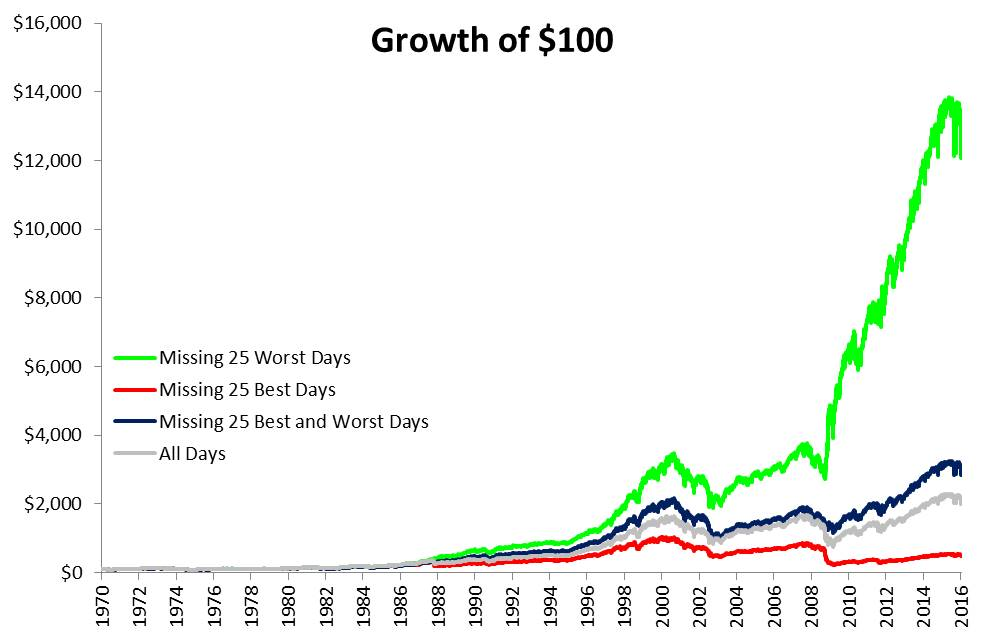
\includegraphics[width=0.6\textwidth]{beststockdays}    
 %  below is only a naming convention, above is the real deal
    \label{fig:beststockdays}
	\caption*{\small Source: Market Watch\cite{bestdays}}
\end{figure}

\subsection{Machine Learning Model Description}

\subsubsection{Artificial Neural Networks}
Artificial Neural Networks (ANN) were conceptually first written about in the early 1940s \cite{Widrow1990} when neurophysiologist Warren McCulloch and mathematician Walter Pitts wrote a paper on the theoretical functioning of neurons. Donal Webb then expanded on this in his paper "The Organization of Behavior" while the first computerised neural networks were developed by IBM in models called "ADALINE" and "MADALINE" \cite{Widrow1990}. At their core, ANNs are a series of large matrix multiplications where weights and biases, which represent the strength of connections between nodes, are optimized to provide the best approximation to the desired output.\par The popularity of ANN methods have increased as enhanced computational power led to the lowering of barriers to entry in the field. One of the more popular networks used in practice is the mutlilayer perceptron, initially introduced by Frank Rosenblatt in 1958 \cite{Rosenblatt1958}. A perceptron is the simplest form of a layered network and consists of a single neuron with an adjustable weight. The perceptron can divide the hyperplane into a 2-dimensional space which is then used to classify the given inputs. The hyper plane is defined by the linearly separable function below.

\begin{align}
\sum^{n}_{i = 1} x_{i}w_{i} - \theta = 0  
\end{align}

Multi Layered Perceptrons (MLP) can be defined as 
\begin{align}
NeuralNet^{l}_{j} =  \sum^{N_{l}}_{i = 1}w^{l-1}_{ij} y^{l-1}_{i}  
\end{align}
where $NeuralNet^{l}_{j}$ is the $l$th layer of the $j$th neuron which gives us the weighted sum of its inputs. The weights of the connections to the next layer $l=1$ are used to calculate the weighted sum of inputs for the subsequent layer in the network.  \begin{align}
Y^{l}_{j} =  ActivationFunction(NeuralNet^{l}_{j})  
\end{align} 
This weighted sum of inputs is then passed through to an activation function which maps the output of the hidden layer to a space defined by the activation function, in this step we can introduce non linearity into the model itself by using a non linear activation function such as the softmax function described below (which is used in this project for the recurrent neural network model (RNN) ).
\begin{align}
y =  \frac{\exp(x_{i})}{\sum^{k}_{j=0}\exp(x_{j}) } \quad for \  i = 0,1,2,..k
\end{align} 
This maps any series of values onto a plane of [0,1] and the output depends on the values produced by the node which feeds the activation function. \par While there are a vast array of model training techniques , one method to train an ANN is to use backpropagation, where updates to the network's weights are fed backwards through each layer. Each model has an error function which is used to grade performance, which could be the the squared difference between the models output and the desired output (mean squared error, used in training the RNN in this project).  \newline The universal approximation theorem \cite{Kurkova1992} of the MLP model in neural networks states that ANNs can approximate any function and thus in theory, should be able to identify any patterns within the data that another method would also identify. \newline The temptation to introduce multiple layers with thousands of connections in order to find a solution is ever present, however (and especially in the realm of finance) this increases the risk of over-fitting or selecting a model based on sheer luck, which fails when tested on live unseen data.
This project uses a recurrent neural network architecture as standard neural networks have limitations. They rely on the assumption of independence among the training and test examples. After processing each data point, the entire state of the network is lost. If the data points are generated independently (such as an individuals medical diagnosis), this presents no problem. But if data points are related in time or space, this approach is flawed.\par In financial assets, the market reacts and learns from the history of the price series, thus data points are indeed related. Recurrent neural networks look promising as they learn the objective function by analysing sequences of points (hence they have been used extensively in text sentiment analysis where context of words within the sentence is important). \par This memory element can be very useful in financial timeseries as past behaviour tends to dictate the future prices path dependancy. The specific model architecture this paper uses is the Long Short Term Memory (LSTM) model \cite{Hochreiter1997}. LSTM has traditionally been used in the prediction of sequences of text in natural language processing. The use of LSTM models in finance is gaining popularity with \cite{Fischer2018}, \cite{Lim2019} and \cite{Kucharczyk2019} all using LSTM for time series prediction. LSTM was introduced by Hochreiter et al. in 1997 \cite{Hochreiter1997} and makes use of various "gates" to control the flow of information across various nodes.
\begin{align}
{F^{i}}_{t} =  \sigma(W_{F}{u^{i}}_{t} + V_{F}{h^{i}}_{t-1} + bias_{f})
\end{align} 

\begin{align}
{I^{i}}_{t} =  \sigma(W_{I}{u^{I}}_{t} + V_{I}{h^{I}}_{t-1} + bias_{i})
\end{align} 

\begin{align}
{O^{i}}_{t} =  \sigma(W_{O}{u^{i}}_{t} + V_{O}{h^{i}}_{t-1} + bias_{o})
\end{align} 

\begin{align}
{C^{i}}_{t} = {F^{i}}_{t} *{C^{i}}_{t-1} + {I^{i}}_{t} *tanh(W_{C}{u^{i}}_{t} + V_{C}{h^{i}}_{t-1} + bias_{C})
\end{align}

\begin{align}
{H^{i}}_{t} = {O^{i}}_{t}*tanh({C^{i}}_{t})
\end{align}

\begin{align}
{Z^{i}}_{t} = g(W_{z}{H^{i}}_{t} + bias_{z})
\end{align}

where $*$ denotes element wise multiplication, $\sigma$ is the sigmoid activation function, $W$ and $V$ are weights matrices of different layers, and ${F^{i}}_{t}$, ${I^{i}}_{t}$, ${O^{i}}_{t}$ are the forget , input, output gates and ${C^{i}}_{t} $, ${H^{i}}_{t}$, ${Z^{i}}_{t}$ are the cell,  hidden and output states of the LSTM. The LSTM uses the cell states to summarise past information and controls the flow of historical memory using the forget gate. The pass through of new information is set by the input gate. Thus the LSTM model should be better equipped than an ANN in learning the long term relationships relevant to assisting in the prediction of the target variable (in this case the future price move). Figure \ref{fig:LSTM_arch} depicts the structure of a Long Short Term Memory Model. 

\begin{figure}[h]
    \centering
% below is where you put the acutal image name in the directory
	\caption{Long Short Term Memory Model}    
	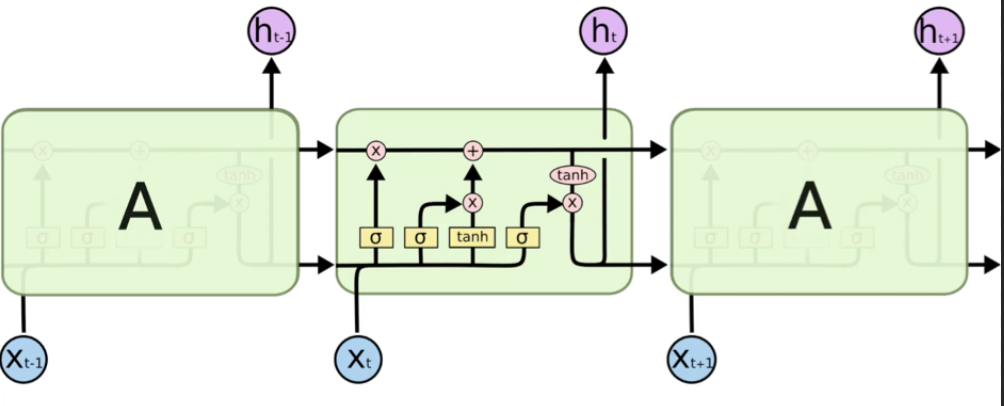
\includegraphics[width=0.6\textwidth]{LSTM_arch}
  %  below is only a naming convention, above is the real deal
    \label{fig:LSTM_arch}
     \caption*{\small Source: colah.github.io, Google Images}
\end{figure}
 
\myparagraph{Background Research}
ANNs have been used extensively in academic financial journals, Czekalski et al. made use of feedforward multilayer perceptrons to predict the direction of the EURUSD currency rate \cite{Czekalski2015}, while Wang et al. applied probabilistic neural networks and  Least Square Support Vector Machine models to assist in the prediction of Chinese equities \cite{Wang2014} . Literature on using ANNs to forecast currencies has a twenty year history as even at turn of the millennium Joarder et al.  tested three separate ANN based forecasting models using standard backpropagation, scaled conjugate gradient and backpropagation with Baysian regularisation to predict movements in various Australian dollar currency crosses \cite{Joarder2003}. Gunduz et al. tested a variety of ANN models and Support Vector Machines (SVM) to try to predict the price of equities traded on the Istanbul Stock Exchange, they found model classification accuracy rates consistently around 70\% on test data \cite{Gunduz2017} . \newline Most of the research cited makes use of various technical indicators which are derived directly from the price series, for example, Gunduz et al. make use of ten price based technical indicators to uncover patterns within Turkish equities \cite{Gunduz2017}. Prior research suggested above 70\% classification rates were attainable on average, however in contrast to this, there is evidence that ANNs often show inconsistent performance on noisy data (\cite{Kim2003},\cite{Kumar2006},\cite{Kim2000}), which highlights the challenges in applying complex models as the risk of overfitting the data remains an ever present threat. 

\subsubsection{Support Vector Machines}
One model which can be used to find patterns in financial data are Support Vector Machines (SVM) and Support Vector Regressions (SVR). SVMs were initially introduced by Cortes and Vapnik \cite{Cortes1995} which led to the development of non-linear models which provide binary classifications of target vectors while SVRs output real-valued predictions. In similar fashion to an ANN, the SVM tries to classify an n-dimensional feature vector according to where that data lies on an n-dimensional space.
\newline The model makes use of the kernel trick \cite{kerneltrick} to transform the original data into a higher dimensional space such that we can then uncover a separable hyperplane. The function updates the parameters of the kernel function such that it can more accurately separate and classify the data points. The error correction model in the case of a SVM or SVC (Support Vector Classifier) is a maximisation problem where the model tries to maximise the distance between all the separating hyper planes (maximal margin classifier) it has constructed.  The solution to the optimisation problem can take the form of the following

\begin{align}
Maximise_{\beta_{0}, \beta_{1},...\epsilon_{1}...M}  M_{margin} 
\end{align}
Subject to 
\begin{align}
\sum^{p}_{j=1} \beta^{2}_{j} = 1
\end{align}

\begin{align}
y_{i}( \beta_{0} + \beta_{1}x_{1} + \beta_{2}x_{2} +...+ \beta_{j}x_{ij}) \geq M(1- \epsilon_{i})
\end{align}
such that $ \epsilon_{i} \geq 0$ and $ \sum^{N}_{i = 1} \epsilon_{i} \leq C$. Where $M$ is the width of the margin to be maximised, $ \beta_{i}$ denotes the weight of the coefficients and $x_{i}$ is the $i^{th}$ observation $(i = 1,2,...,N)$ of the dataset, $\epsilon_{i}$ is a variable whose value sets the degree to which individual observations are allowed on the wrong side of the margin or hyperplane. $C$ is a non negative tuning parameter which sets out the total error allowed for observations to be on the wrong side of the margin \cite{James2013}. 
\myparagraph{Background Research}
 Kara et al. utilised SVMs to discover patterns in Turkish equities achieving classification success rates of around 60\% when tested on hold out data \cite{Kara2011}. Both polynomial and radial basis SVMs were trained on a host of price based technical data with the radial SVM outperforming the polynomial SVM. The polynomial SVM also had a much higher variability in classification success rates and thus the radial basis may be best suited to predicting financial time series. The results of the radial SVM were significant with a test statistic of 3 and p-value of 1\%. The radial basis kernel is used in this project.
\newline Similarly, Patel el al. tested a selection of four different machine learning methods (ANN, SVM, Random Forest and Naive Bayes) using ten technical indicators \cite{Patel2015}. The predictor space was also transformed into trend deterministic states, which map the original continuous values into discrete values based on the trend of the continuous valued indicator (downward trend = -1, upward trend = 1). Results suggested that model performance is improved when trend deterministic data is used instead of continuous data. They postulate that the models perform better on the trend deterministic data as this transformation inputs the underlying trend of the indicator which then allows the model to learn the relationship between the underlying predictor trends and the actual output trend.\newline SVM classification rates using this approach (for both radial and polynomial kernels) approached nearly 90\% on average.
Huang et al. also tested the performance of an SVM model (radial kernel) to predict Nikkei futures prices\footnote{Nikkei 225 is one of the main Japanese Stock Market Indices} and achieved classification rates of 73\% on test data. The authors also found that combining model forecasts increased out-of-sample test results \cite{Huang2005}.
Overall, prior research has found interesting and impressive results for using SVMs as a method to predict future time series such as equities (\cite{Gui2015},\cite{Shen2012},\cite{Kim2003}) and currency movements \cite{Kamruzzaman2004}.

\subsubsection{Ensemble Methods: Random Forests}
Ensemble methods are a technique in machine learning which uses the outputs of multiple models to form a consensus around the prediction, while there are many different techniques one can use, this paper proposes to explore whether ensemble methods can be used to reinforce the accuracy of the model on unseen data. One approach is to use tree based methods \cite{Podgorelec2015}, which involve segmenting the predictor space into a number of regions.  Figure \ref{fig:EURUSDMomentum} looks at the prior 12 hour (x-axis) and 24 hour (y-axis) return of EURUSD with the subsequent 24 hour ahead move in the currency colour coded from red (negative return) to green (positive return). 
\begin{figure}[h]
    \centering
% below is where you put the acutal image name in the directory
	\caption{Tree Based Methods Segment the Predictor Space into Numerous Regions}    
	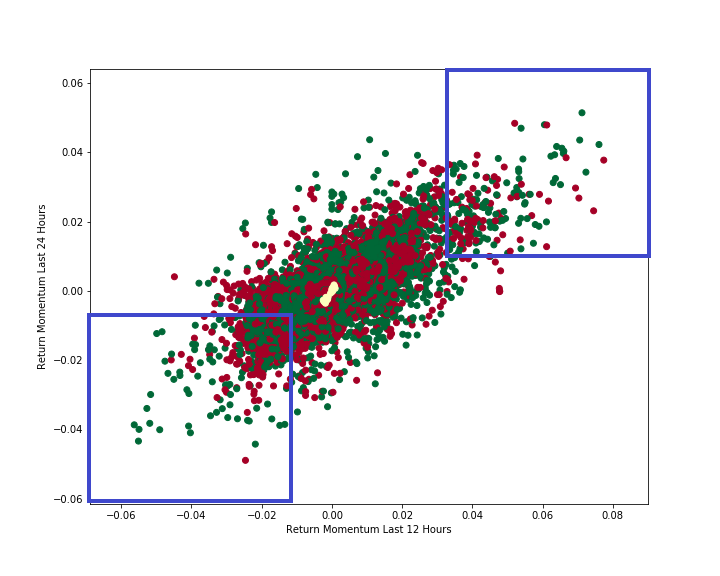
\includegraphics[width=0.6\textwidth]{EURUSDMomentum}
  %  below is only a naming convention, above is the real deal
    \label{fig:EURUSDMomentum}
     \caption*{\small Source: EURUSD FX Rate, Kaggle Database}
\end{figure}
Even in such a simple split of the predictor space, we see some evidence that more subsequent positive days occur in the bottom left of the chart (when prior 12 and 24 hour moves in the currency have been negative). Tree based methods use this type of inference to make predictions on future data points. The goal of the decision tree is to find multiple regions which then minimise the squared error of predictions
\begin{align}
\sum^{J}_{j = 1}\sum^{R_{j}}_{i = 1} (y_{i}-y^{*}_{R_{j}})^{2} 
\end{align}
 where $y^{*}_{R_{j}}$ is the mean response for the training observation within the $j^{th}$ region.
The methods tested in the project will revolve around Random Forests (introduced by Leo Breiman \cite{Breiman2001}) which averages the prediction across hundreds of single decision trees. The trend estimation model uses a random forest architecture to identify trend conducive regimes,
\myparagraph{Background Research}
Research has shown that Random Forests can generalise better than single decision trees as they maintain high variance while reducing the bias of the model\cite{Genuer2012}.
 Random forests use bootstrapping to take multiple random samples from the training data and a random subset of feature vectors to create a diverse array of decision trees which aid model generalisation. This method helps to create decision trees which are uncorrelated to each other and thus have a lower probability of overfitting the data. Patel et al. showed that the it was possible to achieve classification rates of over 80\% for various stock price predictions when using the random forest algorithm and input features which consisted of technical price based indicators\cite{Patel2015}. The research used a random selection of three feature vectors (out of a total of ten) to create each single decision tree in the random forest model and tested the results from 20 to 200 trees using a majority vote for the final classification.  \newline
Kumar et al. performed extensive tests to compare the performance of support vector machines to random forests and found that on average support vector machines outperformed random forests when predicting the direction of the Indian stock exchange \cite{Kumar2006}. Three predictors were considered for each node while the number of trees for each model ranged from 200 to 1500. There was no significant reduction in the error rate for the out-of-sample data based on the number of trees. The RF model achieved classification rates of over 67\% on out of sample data.\newline
Chatzis et al. found that RF methods outperformed SVMs and logistic regression techniques when predicting stock market crisis events, they also note that RF models are relatively robust to overfitting due to each forest only being exposed to a subset of the available feature vectors \cite{Chatzis2018}.
 
\clearpage

\section{Methodology} \label{method}

This section provides a deep dive into the underlying methodology of the full life cycle of the model, including how the data pipeline was structured,  the training and testing methodology and various model evaluation techniques. The model architecture selected was to combine two different models, the first model with the explicit goal of capturing the trend in the time series while the second model would act as a regime identifier and allocate capital to the trend model when the current regime was conducive to the positive performance of trend. The model design is covered in greater detail in section \ref{ProjectD}.

\subsection{System Specifications}
The Python programming language (Python 3.6,\cite{McKinney1976}) will be used as the main programming application to achieve the objectives, with the python packages of Numpy \cite{VanDerWalt2011}, Scipy\cite{Tobergte2013}, Sci-Kit Learn\cite{Geron2017}, Matplotlib\cite{Wood2015} and Pandas\cite{Reiff2002} all providing very useful data manipulation functions to help store, clean and process data. For more complex ANN learning, the machine learning package Keras  \cite{Chollet2015} will be used in the training and testing of Neural network models. In order to train the more intensive models such as the Long Short Term Memory model, a cloud server was used, the specifications of the machine were as follows, 1 CPU with 1.7GB RAM and 250GB SSD. While not computationally very powerful, the machine was selected due to its low running costs which allowed the RNN to train on the dataset overnight. Total time spent running the LSTM model across various training/test periods was over 250 hours. 


\subsection{Data Description}
One of the most important aspects of a trading model is to ensure that the underlying data is of high quality and doesn't contain erroneous values. The trading model uses hourly spot exchange rates for G10 currencies \footnote{Hourly FX Spot Data Provided by Citi Foreign Exchange} alongside various economic data and currency valuation data from the CitiFX and the Organisation for Economic Cooperation and Development (OECD) and national statistics offices.

The data used for this project consisted of hourly foreign exchange data for the EURUSD currency pair\footnote{Value of 1 European EUR in terms of the United States Dollar} and related economic and currency valuation data. Figure \ref{fig:EURUSDMovingAvg} shows the performance of EURUSD over the last sixteen years formed of hourly snapshots and its 55 day and 55 week moving averages. In total the hourly data was sourced from 2001 to the start of 2019, which consisted of just over 120,000 rows of data. One issue encountered was that training the LSTM (even using powerful GPU machines on the cloud server) took a prohibitively long amount of time. This made cycling through various model iterations challenging, with the process often left to run overnight.  There is evidence of the existence of momentum in currencies \cite{Filippou2017} and this project will explore ways of capturing the trending nature of currencies more accurately than a simple linear model.
\begin{figure}[h]
    \centering
% below is where you put the acutal image name in the directory
	\caption{EURUSD Rate Since 2001}
    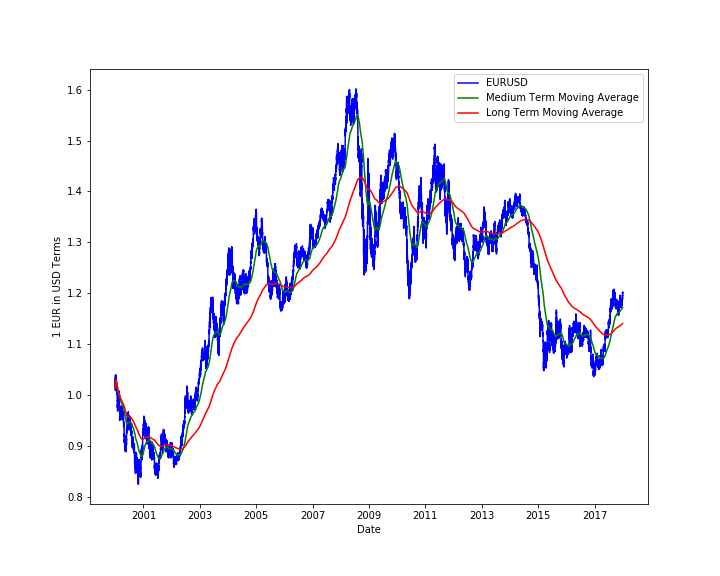
\includegraphics[width=0.7\textwidth]{EURUSDMovingAvg}   
 %  below is only a naming convention, above is the real deal
    \label{fig:EURUSDMovingAvg}
\caption*{\small Source: EURUSD FX Rate, Kaggle Database}
\end{figure}

\subsection{Data Pipeline}

\subsubsection{Objective One: Data Cleaning and Standardisation}
The data was initially screened for errors and missing data points. Cleaning of the data was broken down into outlier detection (to capture any erroneous inputs) and cross checking the data vs known events in time (such as Brexit, election dates) to see if the observed outliers match the expected time frames. This data was also screened and mapped to correct date scales so that the model only used data available at the time of trade signal generation. Once the data had been cleaned appropriately, the next step was to standardise the data and then choose the model features.
 The data was stored and manipulated using Pandas dataframes while Sci-Kit Learn provided the functionality to run both the random forest and support vector regressions. While the package also has some very useful functions such as StandardScaler to standardise the data, in this project a bespoke scaling method was used where the data is standardised by the standard deviation of the feature over a rolling three year lookback window. This is a more realistic approach to use when creating systematic trading strategies as this method uses all available data up to the point of trading and expresses all point in relation to its most recent history, allowing the denominator (the standard deviation ) to vary over time as the market changes regime.
\myparagraph{Standardisation}
Standarising the data remains an important initial step that has been used across a wide variety of prior research. Subtracting the mean and dividing by the standard deviation (z-scoring) \cite{Fischer2018}, min-max standardisation\footnote{Map observations onto a scale of [0,1] with 0 being the minimum value of the observation and 1 denoting maximum} (\cite{Gunduz2017},\cite{Kumar2006})  and other techniques such as  mapping functions to scale feature vectors onto a pre-defined scale (\cite{Kara2011},\cite{Wang2014},\cite{Patel2015}) all help to achieve the overall goal of scaling, which is to ensure that larger or more volatile features do not overwhelm features of smaller magnitude and lower volatility.  Below shows a code snippet of the function to standardise the dataset.
\begin{lstlisting}

def standardise_data(dataset, full_cols, standardised_cols,window):
    '''
    This function computes the standardised returns on a rolling basis looking backwards over the window specified.
    This is the most realistic in terms of a trading strategy and also means the test data is standardised on the correct basis using the
    latest data available at each timestep.
    :param dataframe:
    :param cols:
    :return: standardised dataframe of values
    '''
    train_standardised = dataset[standardised_cols].subtract(dataset[standardised_cols].rolling(window).mean())
    train_standardised = train_standardised.divide(dataset[standardised_cols].rolling(window).std())
    # we will only return the data which is outide the initial window standardisation period
    # add non standardised features
    for feature in full_cols:
        if feature not in standardised_cols:
            train_standardised[feature] = dataset[feature]
    # This function now returns the neccessary file with both standard and non standardised columns.
    return train_standardised.loc[window:,:]

\end{lstlisting}

 \subsubsection{Objective Two: Feature Extraction}
The model features  were chosen with the goal of capturing the underlying trend of the time series, it is very important in finance that the features are not chosen using a grid search of the hyperparameters. Feature selection driven by mining the training set greatly increases the risk of overfitting and should be avoided when working with financial times series \cite{Arnott2018}. Thus the features which had an intuitive justification for defining the trend are shown in the following table. Financial time series prediction is a very challenging task given the inherent noise in the data, thus the number of available features were kept to a minimum and in effect used only the deviation of the currency price from the short, medium and long term price averages. We use these features as they allow the model to capture the underlying trend (in either an upward or downward direction) by looking at the current price level in relation to historical levels.

\begin{table}[h] 
\centering      % used for centering table
\caption{Model One: Trend Capture} % title of Table 
\resizebox{\columnwidth}{!}{% 
\begin{tabular}{l l l}  % centered columns (3 columns) 
\hline                     %inserts double horizontal lines 
Indicator & Description &  Type \\ [0.5ex] % inserts table %heading
 \hline                    % inserts single horizontal line 
Short Term Momentum & 5,10, 21, 55 Period Moving Average & Technical \\   % inserting body of the table
Medium Term Momentum & 100, 155, 200, 255 Period Moving Average  & Technical \\ 
Long Term Momentum & 300, 350, 400, 455 Period Moving Average  & Technical\\ 
\hline     %inserts single line 
\end{tabular} %
}
\label{table:feature} % is used to refer this table in the text 
\end{table} 
The following formula was used to calculate the deviation of the current price to its moving average over a set horizon. This project used an exponentially weighted moving average.
 
\begin{align}
EMA_{t} = price_{t}*k + EMA_{t-1}*(1-k) \quad for \ i = 1,2,3...t
\end{align}
where $k = \frac{2}{(N+1)}$ , and $N$ is the length of the moving average and $price_{t}$ is the price of the underlying asset at time, $t$.\par 
Dimensionality reduction (via principle component analysis) was also performed on the features, however this did not have any positive impact on the models performance.
\myparagraph{Feature Selection For Trend Regime Prediction}
The feature selection process for model two (estimating the likelihood of a trending price series) was based on economic intuition as this can lessen the probability of over-fitting \cite{Arnott2018}. As patterns and correlations in prices can change quite quickly, it is important not to overfit the model on the training data.  The technical price based indicators are captured in the first model, while the second model measures non-price based information such as economic momentum and risk appetite (which is a measure of markets current sentiment). 
Table \ref{table:feature} outlines the features which will be used in model two.
\begin{table}[h] 
\centering      % used for centering table
\caption{Model Two: Trend Strength Estimation} % title of Table 
\resizebox{\columnwidth}{!}{% 
\begin{tabular}{l l l}  % centered columns (3 columns) 
\hline                     %inserts double horizontal lines 
Indicator & Description &  Type \\ [0.5ex] % inserts table %heading
 \hline                    % inserts single horizontal line 
Relative Economic Momentum & 1 Year Economic Momentum & Economic\\ 
Global Economic Momentum & 1 Year Global Economic Momentum & Economic\\
Currency Volatility & Annualised Volatility & Technical Stress Factor \\[1ex]
\hline     %inserts single line 
\end{tabular} %
}
\label{table:feature2} % is used to refer this table in the text 
\end{table} 

The approach of combing two separate models each with specific goals is a novel way to use machine learning in finance, in essence one model controls the price prediction component while the second model is used to gauge how likely the first model is to generate positive returns.

\subsubsection{Justification of Features} \label{justify}
The aim of the features used in this project was to try to juxtapose higher frequency technical price data alongside lower frequency economic data to assist in a model's prediction accuracy. While price based metrics offer the easiest route to higher frequency data, they also lack the ability to capture the fundamental economic factors that can drive currency direction \cite{medium}. Thus combining two separate models to handle each aspect of the trade signal process can create synergies between each model. 
Below we showcase factors that can impact currency direction.
\myparagraph{Economic Fundamentals} 
One of the most important factors that sets the broad direction of a currency pair is the relative economic performance between two countries.
Dahlquist et al. show that measuring relative economic momentum between different countries has the ability to forecast currency direction over medium term horizons \cite{Dahlquist2015}. That paper showed statistically significant results that economic fundamentals have an important role in relative capital flows and subsequent currency direction. This economic feature is used in model 2 to capture relative economic dispersion between the Euro Area and the United States, with the view that diverging economies should create an environment where currencies trend in the direction of the economic outperformance. 
\myparagraph{Price Momentum}
Price momentum here refers to the historical trend in the currency,  research does suggest there exists  exploitable momentum within the currency space \cite{Moskowitz2012}. The reasoning for the existence of momentum in currencies is likely due to decision delays amongst different investor segments who build up positions in currencies over time. Auto-correlation in currency returns may also exist as information is priced slowly over time (such as economic data) and thus as more economic data is published, this adds further confirmation to a trading signal and thus conviction and trade size increases. Model one is tasked with capturing price momentum.
\myparagraph{Risk Appetite}
Risk appetite in financial trading refers to the wider investor communities appetite for higher risk assets. For example when risk appetite is high, then investors buy equities and currencies with high interest rates as they are happy to take the higher probability of losses (.i.e. the investment risk) associated with the higher return. Aggregated global economic data help to forecast changes in risk appetite as investors react positively to strong global growth and negatively to global growth shocks. Low risk appetite (growing investor fear) tends to be accompanied by regime shifts, and also increases in price momentum as the asset searches for a new equilibrium price level. Model two uses this feature for regime prediction.
\myparagraph{Currency Volatility}
The currencies volatility is a measure of how erratic the currency is behaving and increases in currency volatility can point towards changing regimes as the market tries to find a new equilibrium price level. Model two uses currency volatility as one of the features to assist in identifying a trending regime.
\vspace{5mm}

While the above drivers of currency markets are not exhaustive, it can provide a frame work for constructing a systematic trading strategy. Currency drivers can shift over the short and medium term and while this can all be partially captured by price action, it is also prudent to try to understand the dynamics of other potential drivers as discussed in the previous section. \newline
Therein lies the main problem when combining machine learning and finance, that other areas such as the biological or physical sciences do not encounter, is that at the core of each price, are human or human created trading algorithms which have collectively decided on a price level at which to transact. \newline Every price of a trade in financial markets consist of the dreams, fears and greed of human emotion. Not only this, but market investors are influenced by past patterns and incorporate new information (including newly published research) into future decisions, thus altering the environment in which the historical pattern has been learned. Bartram at al. provide evidence that anomaly (excess) profits published in research papers tend to decay substantially in the period after publication, which suggests any new findings are arbitraged away\footnote{Of course a more sinister reason could be model overfitting on historical data} quickly as the new information is incorporated into the market\cite{Bartram2019}. \par

While early academic research espoused the efficient market hypothesis, there are certain times where the market is not fully rational \cite{Dome2008}. Thus opportunities do exist, but finding repeatable trading opportunities requires more than just analysing price patterns in data. Given the randomness of markets, even poor strategies can perform well for long periods of times due to sheer luck. This creates new challenges for practitioners of machine learning in finance, in fact, new research has also started to focus on protocols and best practices around data mining in finance \cite{Arnott2018}.

Being able to identify trends and trend regimes would allow the trading model architecture to outperform other simpler linear models while not churning (over trading) the portfolio if currency starts to enter a pattern of mean reversion. Building the model to this asymmetric specification can assist in the generalisation of the model. \newline Thus it was decided to first train a model to identify trends in each series and then overlay that model with another capable of using the non-price data to identify periods when currencies exhibit trending behaviour. For example, periods of elevated economic dispersion could be conducive to trend strategies outperforming.

\subsection{Objective Three: Training and Testing Methodology}
The model training stage allows the learning algorithm to understand and capture the relationship between the features and the classification target vector (the target vector will be the future direction of the asset price 24 hours in the future). Prior research has generally used binary classification of the future asset price move when developing models(\cite{Abreu2018},\cite{Gunduz2017},\cite{Chatzis2018}). \newline Model training allows us to understand which combination of models (RNN, SVM, RF) and underlying architecture (hidden layers, number of decision trees, kernel type) are best suited to capturing the nuances in the data. This stage of the process also provided an opportunity to experiment with various models to see the differences in performance. The training and testing phases were performed over multiple different windows such as walk forward testing, K-fold testing \ref{fig:Train_Test} and simple train and test splits over the full dataset. The structure of the different training/testing methods are shown below. The results of training and testing on the price data will be further explored in section \ref{results}. The code below shows a snippet of a python function called create\textunderscore train\textunderscore  test file written to split the data set into various train and test periods based on whether one wants k fold training or walk forward training.

\begin{lstlisting}
    # training size is the first x data points and the test data is appended onto the train data 
    # such that we use a walk forward testing framework
    if concat_results:
        # provide data up till the test data zone
        train_data = int(data_file.shape[0]) - (test_size + test_buffer)
        train_original = data_file.iloc[:train_data, :].reset_index(drop= True)
        # provide data in the last x points of test data available
        test_original = data_file.iloc[-test_size:, :].reset_index(drop= True)
    else:
	# this effectively acts as a batch training/split
        train_original = data_file.iloc[:int(data_size), :].reset_index(drop= True) 
        test_original = data_file.iloc[int(data_size) + test_buffer: (int(data_size) + int(test_size)), :].reset_index(drop= True)
\end{lstlisting}
\vspace{4mm}
\begin{figure}[h]
    \centering
% below is where you put the actual image name in the directory
	\caption{Walk Forward and K-Fold Train/Test Split}    
	\includegraphics[width=0.5\textwidth]{Train_test}
  %  below is only a naming convention, above is the real deal
    \label{fig:Train_Test}
     \caption*{}
\end{figure}

\subsection{Objective Four/Five: Model Evaluation Methods} \label{backy}
In order to validate the model, the standard procedures of analysing the mean-squared error, classification hit rates and precision and recall will be analysed. However, given this is a trading system, the selected model and its structure will need to be tested in a similar setting to real world trading. This requires the construction of a backtesting engine which can simulate each models performance taking into the signal lag \footnote{ The time between signal generation and trading time} and the currency performance per each trading signal. This will provide a much more accurate analysis of the selected trading strategy performance\footnote{The vast majority of research papers referenced in this thesis did not perform this type of testing}. While classification success rates will be important in gauging model accuracy, high classification rates may not lead to positive strategy performance if large currency moves are mis-classified. A code snippet taken from the trade backtesting engine is shown below .
\clearpage
\begin{lstlisting}
def backtester(results, test, trade_horizon):
    '''
    Calculate the returns of the trading strategy and store the results in the test file.
    :param results: the trading signals generated by the model.
    :param test: this contains the test data
    :param trade_horizon: this is the length of time of the trading signal prediction
    :return: A dataframe which has the test data and also the results of the trading strategy in pct terms of log returns.
    '''
    # This needs to change to handle the change in the target
    predictions = pd.DataFrame({"Date": test['Date'], "Predictions": results})
    test_results = pd.merge(test, predictions, how="left", on="Date").fillna(0)
    # calculate the returns of the signal for the signal which has been put through the error function to smooth the position.
    test_results["erf_signal"] = test_results['Predictions'].apply(erf)
    test_results["scaled_signal"] = test_results['Predictions'].shift(2).rolling(trade_horizon).sum() / trade_horizon
    test_results["scaled_signal_erf"] = test_results['erf_signal'].shift(2).rolling(trade_horizon).sum() / trade_horizon
\end{lstlisting}

\subsubsection{Assessing Model Performance}

\paragraph{Mean Squared Error}
The mean squared error (MSE) is used to measure the prediction accuracy of the model. It looks at the average distance of the predicted value from the actual value.
\begin{align}
Mean Squared Error = \frac{1}{N}\sum^{n}_{i = 1} (y_{i}-F(x_{i}))^{2} 
\end{align}
where $y_{i}$ is the actual value and $F(x_{i})$ is the predicted value for the $i_{th}$ observation. Normally it is best practice to choose the model which has the lowest test MSE. \newline
\paragraph{Precision and Recall}
Another method of model validation is to look at the precision and recall of the model \cite{Patel2015}, whose values can be calculated from a confusion matrix, which shows the number of correct and incorrect classifications per class. Table \ref{table:confusion}  shows the confusion matrix for a two class classification problem.
\begin{table}[h] 
\centering      % used for centering table 
\caption{Confusion Matrix} % title of Table 
\resizebox{.75\textwidth}{!}{%

\begin{tabular}{l l l}  % centered columns (3 columns) 
\hline                     %inserts double horizontal lines 
Actual (row) Predicted (col) & Buy &  Sell \\ [0.5ex] % inserts table %heading
 \hline                    % inserts single horizontal line 
Buy & True Positive & False Negative \\   % inserting body of the table
Sell & False Positive & True Negative \\ [1ex]
\hline     %inserts single line 
\end{tabular} %
}
\label{table:confusion} % is used to refer this table in the text 
\end{table} 

The confusion matrix allows us to calculate the precision and recall of the model.
\begin{align}
Precision = \frac{True Positive}{True Positive + False Positive} 
\end{align}
\begin{align}
Recall = \frac{True Positive}{True Positive + False Negatives} 
\end{align}
The precision captures the correct positive signals ( e.g. in this case the correct number of buy signals as a percentage of all buy signals) that were actually triggered. Recall measures model accuracy as a function of the total number of positives in the data set itself. These statisitcs are important to analyse when assessing trading models as certain periods can be heavily biased towards one class, for example in the case of a financial asset which has a strong trend will by design have a higher occurrence of one class vs another.

\paragraph{Deflated Sharpe Ratio}
Given the inherent issues of overfitting in finance (\cite{Arnott2018},\cite{LopezdePrado2018}), it is also important to analyse the overall Sharpe Ratio \cite{Sharpe2009} which measures the return of a trading model per unit of risk (or volatility of returns). \newline High Sharpe ratios can be obtained by a genuinely good prediction model or through pure overfitting/selection bias, hence it is useful to deflate the Sharpe Ratio of every strategy tested to take into account the number of model tests as well as the skew of each strategy's distribution \cite{Bailey2014}. 
The Deflated Sharpe Ratio is a test statistic which can outline the probability of having found a true positive. It is defined below as
\begin{align}
\widehat{DSR} = \left[
		 				\frac{\widehat{SR}-\widehat{SR_{0}}\sqrt{T-1}}
						{\sqrt{1-\gamma_{3}\widehat{SR} + \frac{\gamma_{4} - 1}{4}*\widehat{SR}^{2}}} 
				 \right]
\end{align}
where $\widehat{SR}_{0} = \sqrt{V\left[\widehat{SR}_{n}\right] 
						\left(      	
							\left(1- \gamma\right) Z^{-1} \left[ 1- \frac{1}{N}\right] + \gamma Z^{}-1 \left[ 1-\frac{1}{N}\exp^(-1) \right] 
						 \right)}$
and $\widehat{SR}$ is the estimated Sharpe Ratio to be tested, $T$ is the sample length, $\gamma_{3}$ is the skewness of the returns distribution and $\gamma_{4}$ is the kurtosis of the selected strategy,  $V\left[\widehat{SR}_{n}\right]$ is the Sharpe Ratio variance across the number of strategies tested, $N$ is the number of independent trials of strategies run (.i.e. the number of models tested) and $Z$ is the cumulative function of the Gaussian distribution\footnote{Further information and theoretical proofs of the deflated sharpe are available from \cite{Bailey2014}}.  

\clearpage

\section{Project Design and Implementation} \label{ProjectD}
This section outlines the specific steps taken to create each model and provides some justification for the selection of various model parameters and specifications used.
Various Python packages such as Sci-Kit Learn and Keras were used to create and test the classification success rates of each type of model. Fischer et al. made use of Keras (on top of Google's Tensorflow) to implement Recurrent Neural Networks (RNN) \cite{Fischer2018} while using Sci-Kit Learn for logistic regression, SVM and Random Forest methods. \newline One issue encountered was that the length of time needed to train the LSTM meant that training multiple variations across parameters was challenging from a time perspective. 
\subsection{Model Architecture}
Three model architectures were used in this project.
\begin{itemize}
 \item Recurrent Neural Networks: Long Short Term Memory Models
\item Decision Trees: Random Forests.
\item Support Vector Machines: both classification and regression methods. 
\end{itemize}
One novel approach in selecting the target vector (.i.e. the future return of the asset) was to used a risk adjusted return and predict the risk adjusted return as opposed to the binary return \cite{Lim2019}, this ensures that the trend model can also estimate the positioning size and negates the need for a separate trade risk adjustment to be made. \newline
 
During the course of the project, it became clear that using historical price data to train the model produced erratic performance in the testing period across all three models and various training and testing phases. Perhaps this was due to the nature of the underlying security being EURUSD (one of the most highly traded instruments in finance and thus was highly efficient) or that the model tended to over fit the training data (even when using techniques such as drop out rates and tree pruning was performed). 

\subsubsection{Trading Model Methodology} \label{rand}
The failure of the model to learn robust profitable trading patterns using its own price data was one risks cited in the proposal which came to fruition. The solution to this problem was to switch the model from one which trained on the actual price series to one which trained on randomly generated price data which had a built in a trend component. In effect it was necessary to go back to basics and understand what the goal of the model and its features ultimately was, trend prediction.\par
If the series we are trying to predict has only exhibited trend in patches across the full time frame of available data, then the model is likely unable to pick this trend up over the full sample, as it ends up training on conflicting patterns. Figure \ref{fig:train_test_periods_matter} tries to illustrate this point, showing a sucessful training and test period for EURUSD, and also an unsuccessful period , where the training occurs on a period without any trend, while the test period is then a regime of strong trend.This type of issue emerged when training using K fold cross validation. In some instances the training data set happened to be during regimes of strong upward or downward trends, and subsequently the model would perform well in the test phase\footnote{The results of various model performance is covered in section \ref{results}}. 
\begin{figure}[h]
    \centering
% below is where you put the acutal image name in the directory
	\caption{Do you Feel Lucky? Model Performance Impacted by the Selection of the Training Period}    
	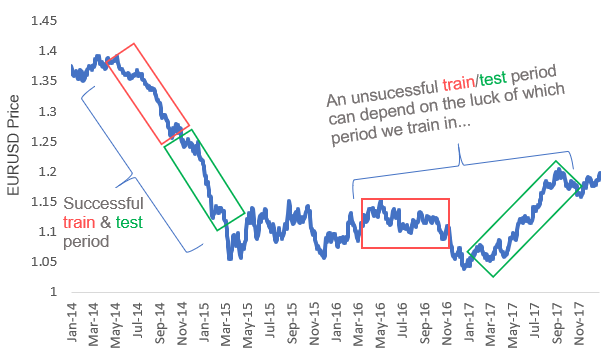
\includegraphics[width=0.6\textwidth]{train_test_periods_matter}
  %  below is only a naming convention, above is the real deal
    \label{fig:train_test_periods_matter}
     \caption*{}
\end{figure}

Thus for the model to be able to capture trends, it needed to be trained to \textit{recognise}a trend, therefore, a decision was made to switch the training data away from the historical price series data and onto randomly generated trending data series which could replicate trends in asset price series. Of course when training on randomly generated data one must also include some noise term such that we create series which mimics financial asset prices. Hence the trending data was injected with a noise term.
Training on randomly generated data has two very appealing traits, one it reduces the chances of overfitting the data, however this is reduced but not removed as there is a chance the randomly generated data series happens by chance to mimic closely the testing phase of the data (hence training of various iterations of the randomly generated data is important). Secondly, it opens up the full live price series data to exist as the test dataset. By training the model to recognise trends, we can now test on the full 120,000 rows of EURUSD price data. 

The randomly generated price series was created using the following formula.

\begin{align}
X_{t} = X_{t-1}*\alpha + \epsilon_{t-1} 
\end{align}

where $X_{t}$ is the simulated price at time $t$ , $\alpha$ is a parameter to control the strength of the trend and $\epsilon$ is a randomly distributed i.i.d error term used to simulate the noise of financial time series.

The trend capture model (model one) is described in the below diagram \ref{fig:TrendCapture}. The figure outlines how the underlying features feed into the trend model and also how each selection of features are tailored to capture short, medium and long term trend frequencies. Model one handles the signal generation process, by measuring the underlying relationship between the features and the target return variable. As mentioned in \ref{table:feature}, the features were created from price based technical signals, such as deviations from exponential moving averages across both short, medium and long frequencies. This purely price based factor model is used to capture trend only, hence we feed in only factors which are applicable to signaling a trend in either direction.  

\begin{figure}[h]
    \centering
% below is where you put the acutal image name in the directory
	\caption{Model Architecture : Trend Capture}    
	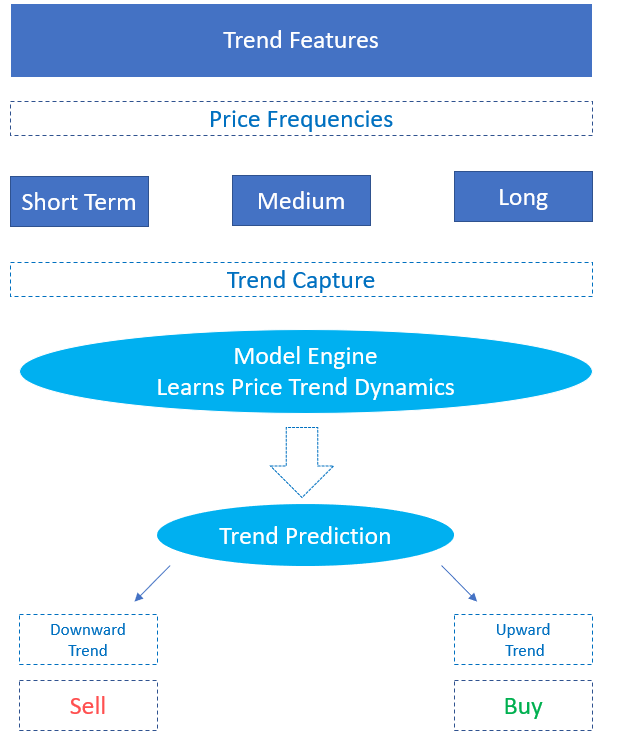
\includegraphics[width=0.6\textwidth]{TrendCapture}
  %  below is only a naming convention, above is the real deal
    \label{fig:TrendCapture}
     \caption*{}
\end{figure}
 The overall goal of model one is to use machine learning models to identify the pattern and non-linearities inherent in trending prices which more simple linear based models fail to capture.  The type of model also varied from using regression methods to estimate a continuous valued 24 hour period ahead and also a more simple classification on whether the price was predicted to move higher or lower. This one day ahead trend prediction was then used as the input into model two (trend estimation, \ref{fig:TrendEstimation}).
\clearpage
The second model (figure \ref{fig:TrendEstimation}), then tries to capture the prevailing market regime, and uses much slower moving fundamental data as features (as described in \ref{table:feature2}) in order to assist in position sizing of the trend model, by learning when historical fundamental features have tended to coincide with the positive performance of the trend strategy. This work on the intuitive reasoning behind why a currency exhibits trending behaviour, one process of thought is that economic dispersion between countries \cite{fxalpha} can lead to large trends between currencies as the capital is pulled towards the currency of the economically stronger country. Decision delays by different segments of investors can also influence the slow grind of a higher price, while central bank monetary policy can also lead to large deviations between different countries currencies. Central bank policy can often be driven by economic data and thus looking at economic data we maybe able to identify regimes which are conducive to trending prices series. We also include a volatility feature as well as global and G10 economic performance, which can act as a potential harbinger of further increases in volatility when trend is driven by factors such as risk appetite (where investors flock back to safe haven assets). The target for this model is the performance of the trend model one historically over the testing period. Thus we combine two different models in order to incase the chances of out of sample model generalisation.
 
\begin{figure}[h]
    \centering
% below is where you put the acutal image name in the directory
	\caption{Model 2: Trend Estimation}    
	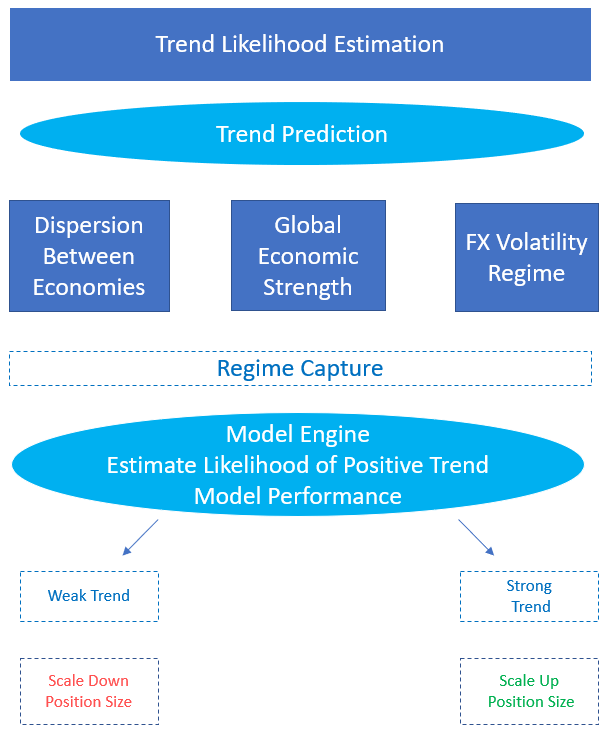
\includegraphics[width=0.6\textwidth]{TrendEstimationv2}
  %  below is only a naming convention, above is the real deal
    \label{fig:TrendEstimation}
     \caption*{}
\end{figure}

\subsection{Machine Leaning Model Parameter Specifications}
As mentioned previously, three different machine learning models were used in the project. The testing and training datasets remained standardised across each model so that comparison of results would be as accurate as possible. The python package Sci-Kit was used to build both the random forest and SVC (SVR) models. Parameter variation was performed across a different number of decision trees and from that analysis, 200 trees where used in the final model phase as it was relatively quick to train and also provided good results (\ref{fig:ntrees}). When looking at the results of batch training and testing, we can see that adding more trees to the random forest model did not necessarily add more prediction power. Figure \ref{fig:ntrees} shows the mean squared error scores and the sharpe ratio \footnote{assuming a risk free rate of 0\%} of each model trained across various number of trees and using a 50/50 train and test split. The maximum number of features to be selected at each node (i.e. the max features parameter) was kept low to reduce the correlation between trees and increase model generalisation.

\begin{figure}[h]
    \centering
% below is where you put the acutal image name in the directory
	\caption{Random Forest Classifier Performance Across Various Number of Trees}    
	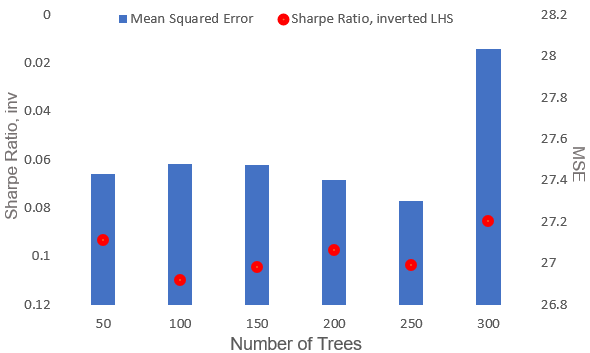
\includegraphics[width=0.6\textwidth]{NtreesMSE}
  %  below is only a naming convention, above is the real deal
    \label{fig:NtreesMSE}
     \caption*{}
\end{figure}

Similarly for the Support Vector regression/classifer models used, a review of the appropriate cost to use was performed. The kernel used was the radial basis kernel to try to capture the non linear patterns in the price series. Interestingly, across various different cost levels, it was noted that higher costs levels tended to have slightly higher accuracy scores which also tended to translate into higher Sharpe ratios in the test period \ref{fig:SVMCost}. The test period of the accuracy scores and Sharpe ratios shown here was from October 2014 until December 2017 ( the period of data post 2017 was truncated at the start of the project to be used for the final blind model testing). Overall, the fact that the higher cost allowances generally performed better in the test period shows the value of not over fitting the training model when using financial time series. 
\begin{figure}[h]
    \centering
% below is where you put the acutal image name in the directory
	\caption{Support Vector Classifier Performance Across Various Cost Levels}    
	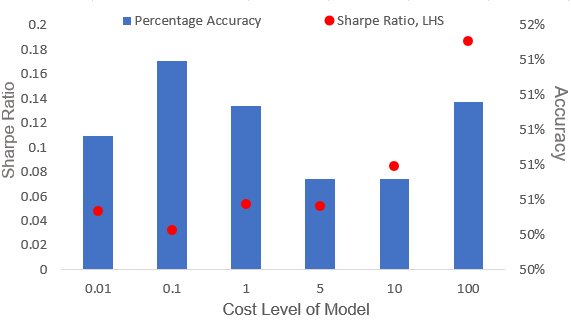
\includegraphics[width=0.6\textwidth]{SVMCost}
  %  below is only a naming convention, above is the real deal
    \label{fig:SVMCost}
     \caption*{}
\end{figure}
The recurrent neural network is one model which is very powerful in terms of the complexity and the nature of problems it can in theory solve, however the increased complexity also comes with a loss of generalisation given the propensity to over fit the data. While this in mind, the following model architecture was chosen to train and test the model, an initial first layer of 32 nodes followed by a layer of 16 nodes where the soft max activation function was used, the model adds a dense layer of eight nodes with a hyperbolic tangent activation function and a final output node which uses a linear activation function. The main parameter which was varied in order to assess model performance was the look back sequence and the number of epochs used to train the model. Generally as the project progressed , the higher the number of training epochs and look back sequences the better the model performance, increasing the epoch and look back sequence size noticeably increased the computational time spent training the model.
\vspace{4mm}
\begin{lstlisting}
   # Initialise the model the Recurrent Neural Network model
    model = Sequential()
    # add a layer of 32 nodes, where the sequences across each observation are returned 
    model.add(LSTM(first_layer,batch_input_shape = (None,look_back,no_features), return_sequences = True))
    # second layer has half the nodes of the previous layer and uses a softmax activation function.
    model.add(LSTM(second_layer, return_sequences = False, activation="softmax"))
    model.add(Dense(8, activation = "tanh"))
    model.add(Dense(1, activation = "linear"))
    # finally the model is complied using the MSE and the adam optimser
    model.compile(loss = "mean_absolute_error", optimizer="adam", metrics = ['accuracy'])
    
\end{lstlisting}
Figure \ref{fig:LSTMlookbacks} , shows the accuracy score and the sharpe ratio (in the testing period) for look back of 25 periods and 66 periods, the 66 period look back outperformed the shorter horizon, possibly as this longer sequence allowed the model to place current price action in the context of a longer window, similar to a human day traders using recent history to base his trading decision on when identifying a trend in the price.
\begin{figure}[h]
    \centering
% below is where you put the acutal image name in the directory
	\caption{LSTM Model Performance Across Lookback Sequences}    
	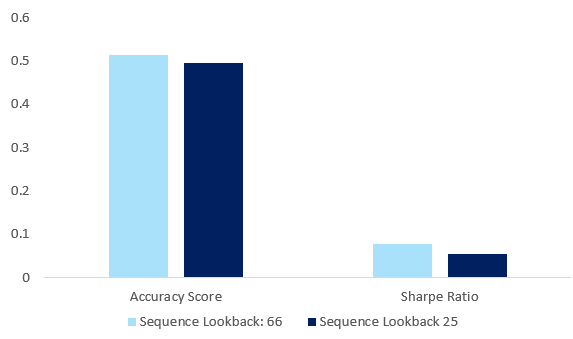
\includegraphics[width=0.5\textwidth]{LSTMlookbacks}
  %  below is only a naming convention, above is the real deal
    \label{fig:LSTMlookbacks}
     \caption*{}
\end{figure}

Figure \ref{fig:500EPOCHTraining_accuracy}, shows the accuracy of the LSTM model on the training data for a given number of epochs. We can see a steady downward slope which initially sees vast improvements in the accuracy scores before it finally settles at a stable if slightly jumpy equilibrium. The training data in this instance was the randomly generated data to mimic an asset price trend, so in this training cycle , the model is learning to understand the features and weights which define a trend in the data. It is this learning process which can then start to recognise trends building in EURUSD in the testing phase.
\begin{figure}[h]
    \centering
% below is where you put the acutal image name in the directory
	\caption{LSTM Model Accuracy Over 500 Epochs}    
	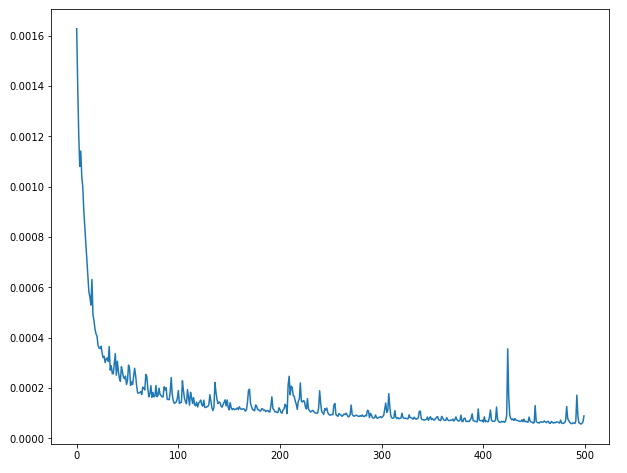
\includegraphics[width=0.5\textwidth]{500EPOCHTraining_accuracy}
  %  below is only a naming convention, above is the real deal
    \label{fig:500EPOCHTraining_accuracy}
     \caption*{}
\end{figure}


\clearpage

\section{Results, Analysis and Discussion}  \label{results}

The initial model training and testing on the EURUSD price series performed poorly, perhaps due to the model overfitting the problem or perhaps due to the different training periods not accurately representing the test data of the model.
In figure \ref{fig:ErraticRetScatter}, we show a scatter plot of the annualised return of trading EURUSD across various machine learning models, train and test periods and model parameters. An acceptable trading strategy needs to be robust and should show clustering of the points despite small tweaks to the model parameters (i.e. showing that varying the strategy parameters does not overly impact the prediction accuracy). In figure \ref{fig:ErraticRetScatter}, we would expect to see a clustering of points near the top left of the chart (which would indicate an area of desirable return per unit of risk taken).  However, we can see points scattered across the chart, suggesting there is a severe lack of robustness in the underlying dynamics of the trading model.

\begin{figure}[h]
    \centering
% below is where you put the acutal image name in the directory
	\caption{Annualised Returns (Y-axis) vs Volatility (X-axis) Across Various Strategies}    
	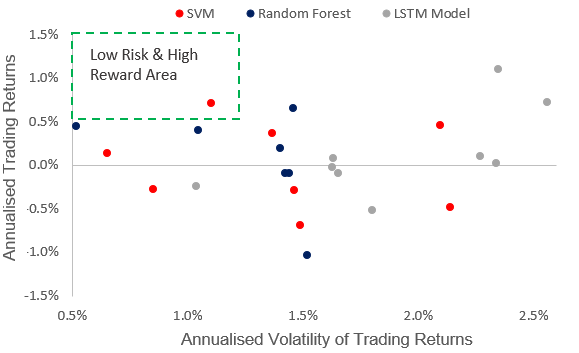
\includegraphics[width=0.6\textwidth]{ErraticRetScatter}
  %  below is only a naming convention, above is the real deal
    \label{fig:ErraticRetScatter}
     \caption*{}
\end{figure}


Figure \ref{fig:model_perf} shows the cumulative return profile for a host of different machine learning trading models across support vector machines, recurrent neural networks and random forests. The returns shown in  \ref{fig:model_perf} display the model performance for various different training and testing periods. The returns are calculated from the backtester outlined in section \ref{backy}. The returns shown on the y -axis are the cumulative log returns of each specific model when trading EURUSD, over randomly sampled 400 day periods. The performance is erratic and scattered across winning and losing strategies. It was due to this under performance and lack of robustness which led to the need to look at alternative model architectures when training the model.

\begin{figure}[h]
    \centering
% below is where you put the acutal image name in the directory
	\caption{Erratic Returns of Machine Learning Based Trading Models}    
	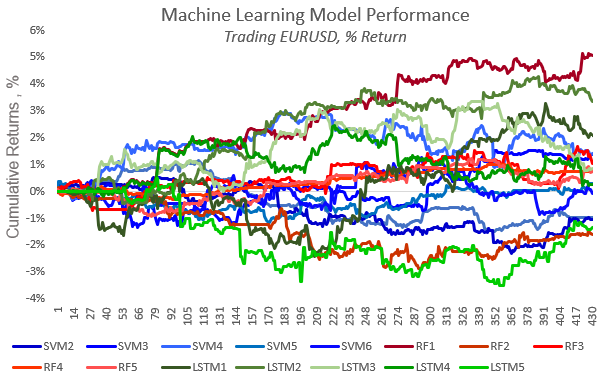
\includegraphics[width=0.6\textwidth]{PoorModelPerf}
  %  below is only a naming convention, above is the real deal
    \label{fig:model_perf}
     \caption*{}
\end{figure}

\myparagraph{Potential Reasons for the Underperformance}
The erratic performance of the machine learning models when training on the price data may be due to the features used or due to the specification of each underlying model. However, given the justification for the features used in the model as outlined in \ref{justify}, one should be wary of using tweaked technical features  solely because they perform better, as that is blatant overfitting. One reason for the erratic performance of each model is that the training period may have occurred in periods where the currency was in a regime of mean reversion or weak trend. This could inhibit the ability of the model to recognise trends. While if the model had trained on a trending price series, then it could learn the patterns associated with the auto correlation in the price, and trade this profitably in the testing period. \newline 
The poor performance of the various models on the live price data in capturing trend was disappointing, however, a decision was made to refrain from running an exhaustive grid search optimisation on the data as this would lead to overfitting of the problem. When one runs multiple simulations across different parameters (especially in finance) then it is inevitable that a profitable strategy is found by luck (similar to a coherent novel being written by a billion monkeys typing randomly on a typewriter). Given the inherent non-stationarity of financial timeseries, it is vital to ensure the model performs in a stable way across a variety of parameters. This rules out extensively applying complex transformations or optimisations on the features as the probability of having selected the "best" parameters by pure chance is high. In financial trading, model robustness is key. \newline As pointed out by Mclean et al.\cite{Mclean2016}, financial model performance can differ vastly prior to publication than after it\footnote{Research suggested a 26\% fall in performance out-of-sample and 58\% decline post publication}, whether due to over fitting or post publication anomaly decay \cite{Bartram2019}, this means we must be extra vigilante when assessing model performance.

Due to this lack of stability in the performance, a different approach was needed. The new approach was to switch the training periods away from the actual price series and towards randomly generated trending data. Using randomly generated price data allows us to calibrate the strength of trend (and the significance of the noise) when training each model on how to recognise trending price series. The goal here is to allow the model to recognise the dynamics and patterns of a trending price series (as the goal of model one is to capture trend only), and thus removes the risk that the training period of the live price series lacks any sustainable trend. The number of data points used to train the models was 50,000 for the Support Vector Machines and Random Forests, while 4000 points were used for the LSTM (in the interest of reducing the time spent training the model). The test data set consisted of the full history of EURUSD data which equated to over 115,000 data points\footnote{Some data is lost due to the rolling standardisation lookback window}. The 24 hour ahead percentage return of EURUSD was the target vector.

\subsection{Performance of Model One: Trend Capture} \label{model1}

This section outlines how various machine learning models performed when trying to predict EURUSD direction having been trained only on randomly generated trending price series. Each of the models here were trained as binary classifiers such that precision and recall could be calculated but also due to the fact that the returns tended to be more robust than when compared to models which predicted continuous variables. This is possibly due to the fact that the regression models tended to be skewed by large values that can occur in financial time series, which meant that when a classifier of the move (up or down ) was used, this helped to dampen the volatility of the signal and removed the impact of outliers on the models ability to learn the patterns of the model.

\subsubsection{Decision Trees: Random Forest}
 The first model tested after training on the randomly generated trend was the random forest machine learning model. Figure \ref{fig:RFRandomDataResults} shows the cumulative log return of trading EURUSD across various iterations of the models trained on different randomly generated datasets. The models below used 200 trees and a maximum of four features when selecting node splits. The testing period here is the full dataset which spans from the start of 2002 to the end of 2017. This testing period covers various different market regimes, such as the Great Financial Crisis, unorthodox central bank policies from 2010 onwards and the end of the commodity super cycle. The model features used were outlined previously in \ref{table:feature}.
\begin{figure}[h]
    \centering
% below is where you put the acutal image name in the directory
	\caption{Cumulative Returns: Random Forest Based Trading Model}    
	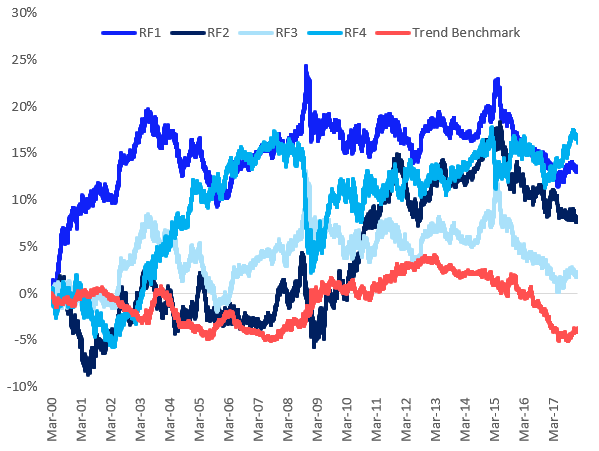
\includegraphics[width=0.6\textwidth]{RFRandomDataResults}
  %  below is only a naming convention, above is the real deal
    \label{fig:RFRandomDataResults}
     \caption*{}
\end{figure}
In terms of results, the returns are still somewhat scattered, however the performance on average is positive. The red line in the chart denotes the performance of a simple linear benchmark strategy of trading in the direction of  the price trend over the last 24 hours, we use this 24 hour period as it matches the trade horizon that the model used as its target variable. Thus the benchmark linear strategy predicts the next 24 hours ahead currency move by looking at what occurred in the previous 24 hours.
\begin{figure}[h]
    \centering
% below is where you put the acutal image name in the directory
	\caption{Performance Statistics: Random Forest Based Trading Model}    
	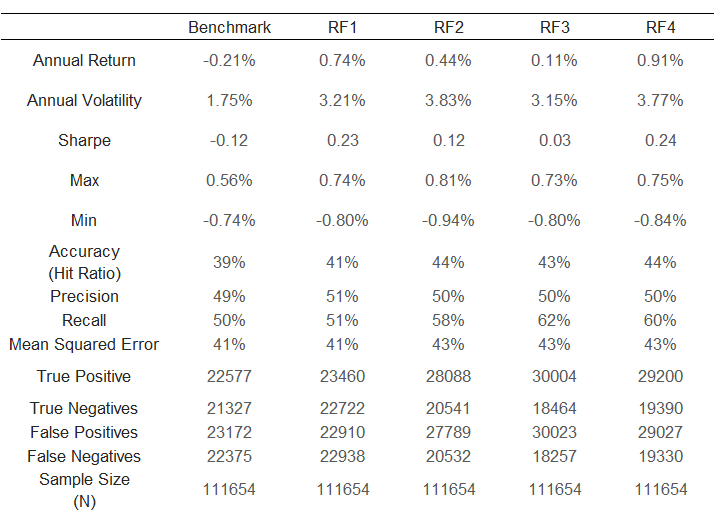
\includegraphics[width=0.8\textwidth]{RFRandomDataStatsv3}
  %  below is only a naming convention, above is the real deal
    \label{fig:RFRandomDataStats}
     \caption*{}
\end{figure}
In addition to the cumulative returns of the strategy, we also shown a break down of each models performance statistics in figure \ref{fig:RFRandomDataStats}, which are broken down to provide the annualised return and volatility, the Sharpe ratio ( risk taken to reward received), the max and min return of each model, the mean squared error (MSE) and the precision and recall. We can see that on average the machine learning models do outperform the benchmark in terms of the MSE, accuracy and Sharpe ratios. The maximum daily return of each model was higher than the benchmark while each ML model also performed better in terms of annualised returns. Overall random forest model was able to identify trending patterns and profitably trade them better than the simple linear benchmark.

\subsubsection{Support Vector Classifiers}
The performance of the support vector classifier was mixed, with some models tending to underperform the simple linear benchmark. As a reminder, the SVC used the radial basis kernael and the train period was 50,000 rows of randomly generated trend data while EURUSD from 2002 until 2017 was the test period. One particular model (labelled SV2 in figure \ref{fig:SVMRandomDataResults},) performed very well up until the final few years of the sample, perhaps as this coincided with a period of mean reverting behaviour in EURUSD. Overall , the SVM model performed somewhat disappointingly over the test full sample.
\begin{figure}[h]
    \centering
% below is where you put the acutal image name in the directory
	\caption{Cumulative Returns: Support Vector Classifier Based Trading Model}    
	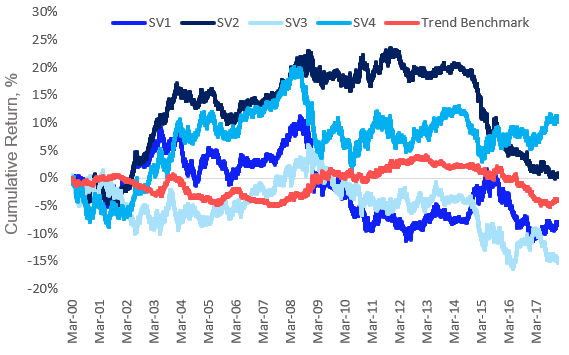
\includegraphics[width=0.6\textwidth]{SVMRandomDataResults}
  %  below is only a naming convention, above is the real deal
    \label{fig:SVMRandomDataResults}
     \caption*{}
\end{figure}

The performance statistics shown in \ref{fig:SVMRandomDataStats} show the under performance of the models in general, as they show low or negative Sharpe ratios alongside underwhelming accuracy rates. The average mean squared error of the SVM models were inline with the linear benchmark.

\begin{figure}[h]
    \centering
% below is where you put the acutal image name in the directory
	\caption{Performance Statistics: Support Vector Classifier Based Trading Model}    
	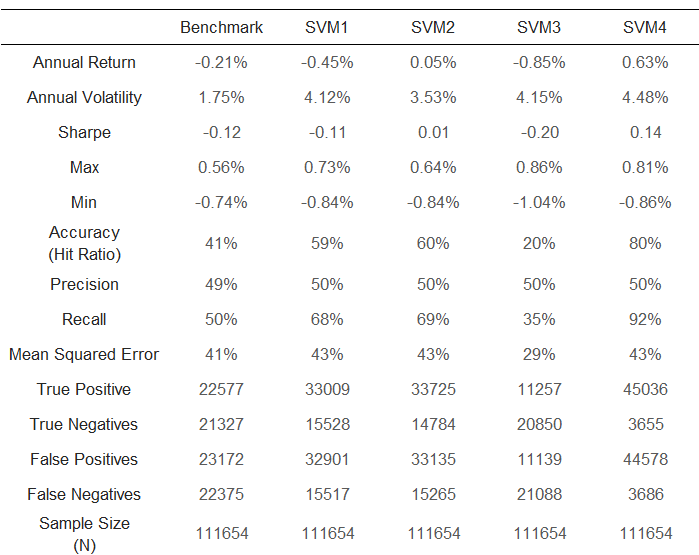
\includegraphics[width=0.8\textwidth]{SVMRandomDataStatsv3}
  %  below is only a naming convention, above is the real deal
    \label{fig:SVMRandomDataStats}
     \caption*{}
\end{figure}

\clearpage
\subsubsection{Long Short Term Memory Trading Model}
The recurrent neural network such as the LSTM provided the most impressive results along with the random forest module, with the majority of models outperforming the linear benchmark \ref{fig:LSTMRandomDataStats}. All of the LSTM models here used an initial layer of 32 nodes , with an additional layer containing 16 nodes and used the softmax activation function. The length of the lookback sequence here was 90 periods while each model was compiled to use the mean square error as the loss function and the "adam" stochastic optimiser. The training period was run over 500 epoch across 4,000 data points. 
\begin{figure}[h]
    \centering
% below is where you put the acutal image name in the directory
	\caption{Cumulative Returns: Long Short Term Memory Based Trading Model}    
	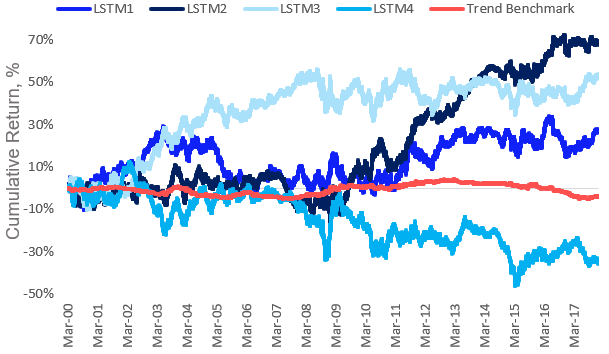
\includegraphics[width=0.6\textwidth]{LSTMRandomDataResults}
  %  below is only a naming convention, above is the real deal
    \label{fig:LSTMRandomDataResults}
     \caption*{}
\end{figure}

The performance statistics \ref{fig:LSTMRandomDataStats} show that the average return across all models  is positive and on a individual basis only model 4 underperformed the linear benchmark in terms of the Sharpe ratio, accuracy, mean squared error and maximum return.  Accuracy, precision and recall scores all ranged from 40\% to above 50\% across all the models, while this is may not seem very good, the fact that the correct predictions outperform the incorrect predictions in terms of percentage return (otherwise the average returns would be negative), then the model does seem to be able to predict the larger moves in the currency. Based on the results, the LSTM models do seem to be best suited to recognising and predicting trends in financial timeseries.
\begin{figure}[h]
    \centering
% below is where you put the acutal image name in the directory
	\caption{Performance Statistics: Long Short Term Memory Based Trading Model}    
	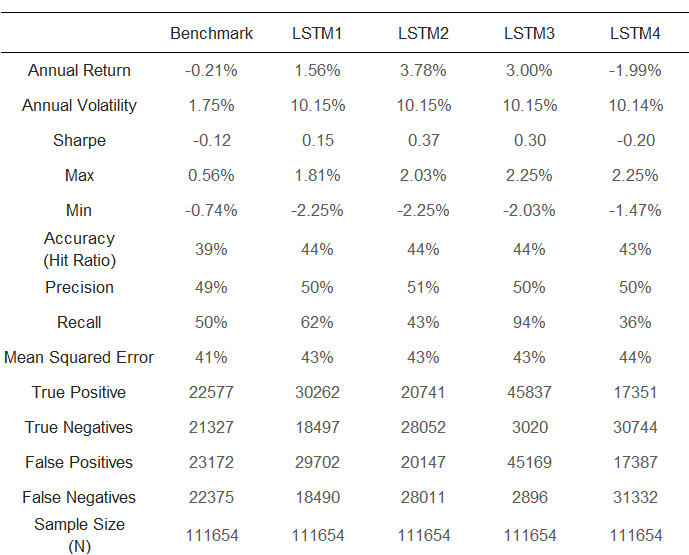
\includegraphics[width=0.8\textwidth]{LSTMRandomDataStatsv3}
  %  below is only a naming convention, above is the real deal
    \label{fig:LSTMRandomDataStats}
     \caption*{}
\end{figure}
\vspace{3mm}
The outperformance of the LSTM model suggests that it is important for the model to understand the historical sequence of the data points such that the patterns of trend can sustain long enough for the model to recognise the sequence of points which form part of a trending price series. This result is also seen in \cite{Lim2019} where the LSTM model outperformed all other machine learning models. Lim et. al used 100 epochs for training \cite{Lim2019}, while in this paper 500 epochs were used to train the model on the randomly generated data, with a sequence look back of 90 periods in the testing phase.

\subsection{Performance of Model Two: Regime Estimation}
This section looks at the performance of the trend estimation model, where we feed in the performance of each trend model (as outlined in \ref{fig:TrendCapture}) and make use of the fundamental features, such as economic growth differentials, historical volatility and the state of global growth to identify periods which can be conducive to the positive performance of trend strategies. The approach taken in this stage of the trading process was split the dataset into one batch training which consisted of the period from 2002 until 2010 and a test period from 2010 until the end of 2017. The model chosen for trend estimation was a simple random forest decision tree as this type of model does not require a large training dataset and can provide important information about the importance of each feature via the variable importance plots. A simplified tree structure is shown for one of the trend models in \ref{fig:decision_tree_model}. In this instance, only three features were used, global economic data momentum, the economic performance differential between the United States and Euro Area and the Economic surprise differential between the US and Euro Area \footnote{An economic surprise measures the difference between the actual economic release value and the economists consensus expectation}.
\begin{figure}[h]
    \centering
% below is where you put the acutal image name in the directory
	\caption{Decision Tree Structure Example of the Trend Estimation Model}    
	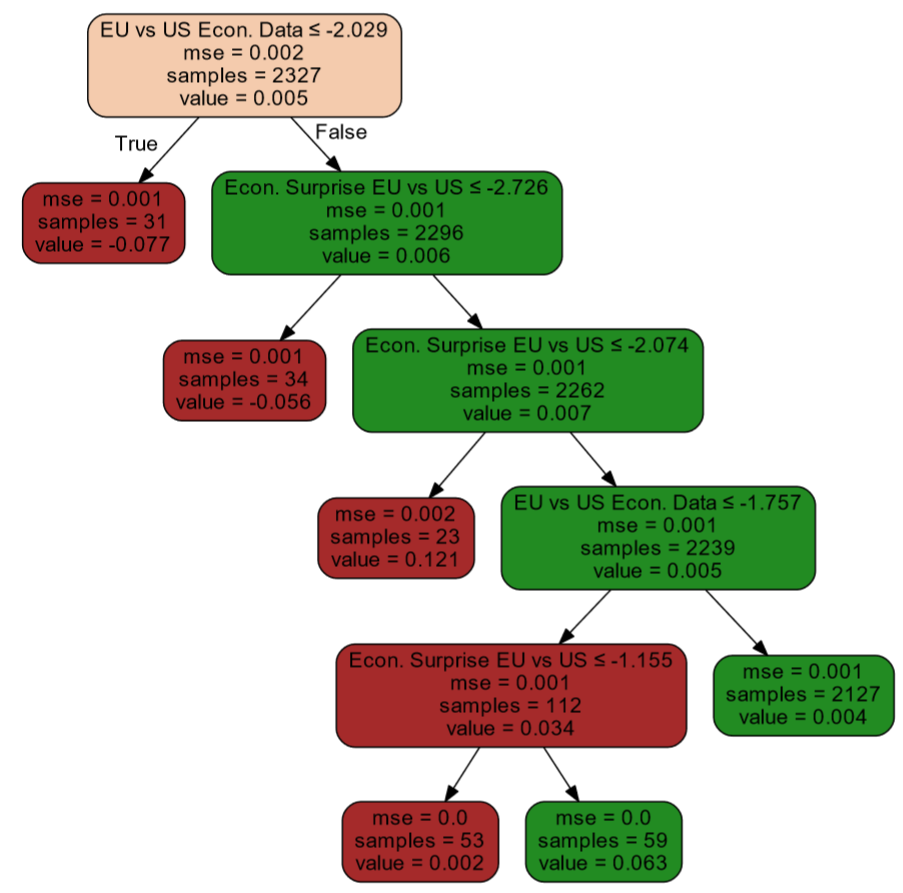
\includegraphics[width=1\textwidth]{decision_tree_model}
  %  below is only a naming convention, above is the real deal
    \label{fig:decision_tree_model}
     \caption*{}
\end{figure}
The decision tree structure of the first split shows that when the economic performance differential between Euro Area and the US has been below -2 standard deviations, then the trend model has under performed. Hence we can see that the goal of the trend estimation model is to align the fundamental factors with periods that the trend capture model has performed well, allowing the second trend estimation model to switch off the trend model when the regime is not conducive to the performance of trend (based on those historical patterns between the trend model performance and the fundamental features).
\clearpage
When running the trend estimation model, given the high number of possible features (and features combinations) across various different lookback horizons, a variable importance plot was created to try to understand which features may have the most explanatory power. A variable importance plot is created by shuffling the features and running the decision tree model each time without one feature to try to uncover how much value that feature adds to the overall prediction ability of the model. \newline  This feature selection study occurred in the training period only. In this case, one trains using daily data\footnote{As fundamental economic data is only available on a daily time frequency} and hence we look to reduce the model dimensionality by selecting a few sub components of the most interesting features. The variable importance chart is shown below in figure \ref{fig:varimp_RF_erf}.

\begin{figure}[h]
    \centering
% below is where you put the acutal image name in the directory
	\caption{Variable Importance Plots of the Features During Training Period}    
	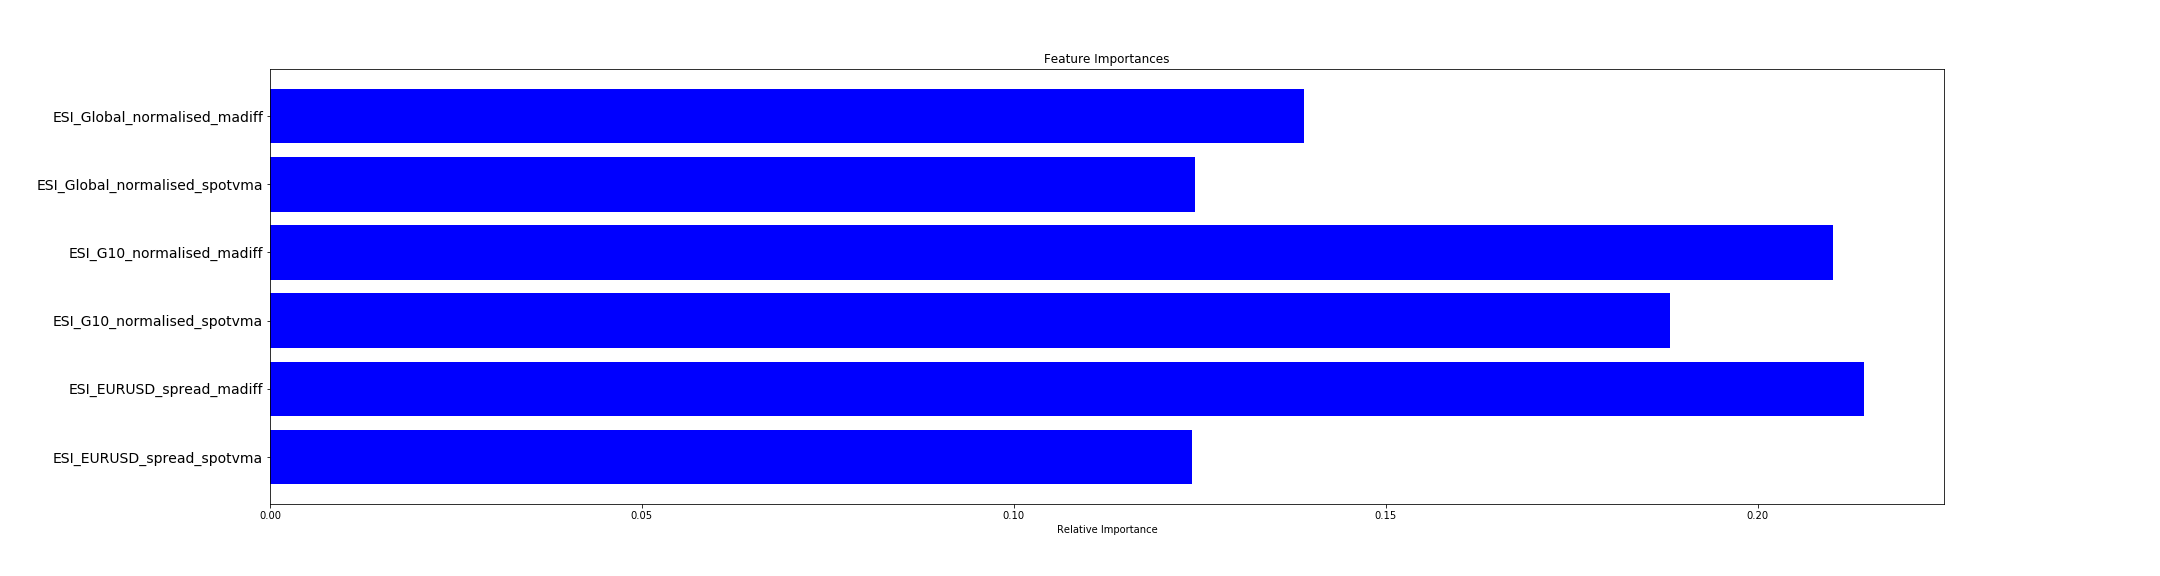
\includegraphics[width=1\textwidth]{varimp_LSTM1_erf}
  %  below is only a naming convention, above is the real deal
    \label{fig:varimp_RF_erf}
     \caption*{}
\end{figure}
We can see that certain features do trend to outperform other features in the level of their predictability. This this allows us to reduce the dimensionality of the model as some of the features are likely redundant. The trend estimation model predicted the performance the trend model one month ahead.  Figure \ref{fig:TrendFilteredResults}, shows the performance of a selection of trend models from each of the three models (RF, SVM, LSTM) which have been fed into the trend estimation model and trained on how each individual model has performed given the economic, macro risk appetite and volatility features shown above.

\begin{figure}[h]
    \centering
% below is where you put the acutal image name in the directory
	\caption{Performance Model 2 Trend Estimation Across Each ML Model Trading Model}    
	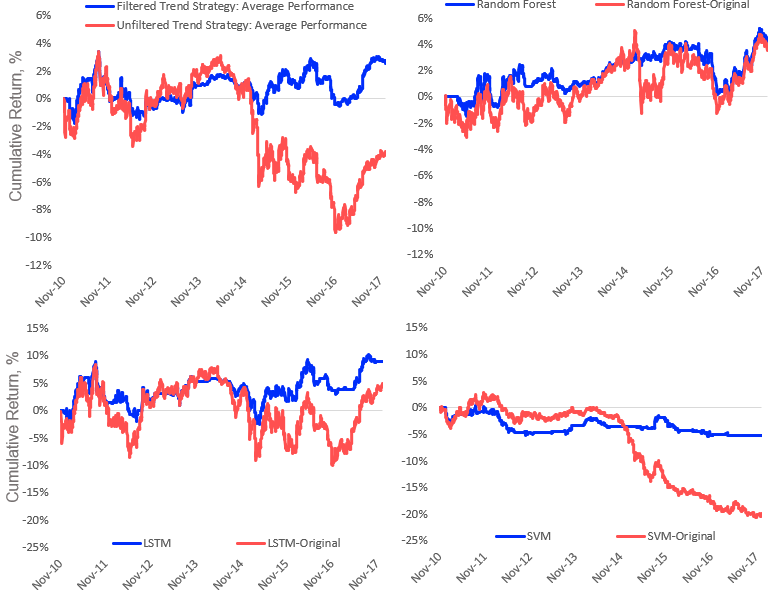
\includegraphics[width=0.7\textwidth]{TrendFilteredResults}
  %  below is only a naming convention, above is the real deal
    \label{fig:TrendFilteredResults}
     \caption*{}
\end{figure}

\begin{figure}[h]
    \centering
% below is where you put the acutal image name in the directory
	\caption{Performance Statistics Model 2 Trend Estimation Average Performance Per Trading Model}    
	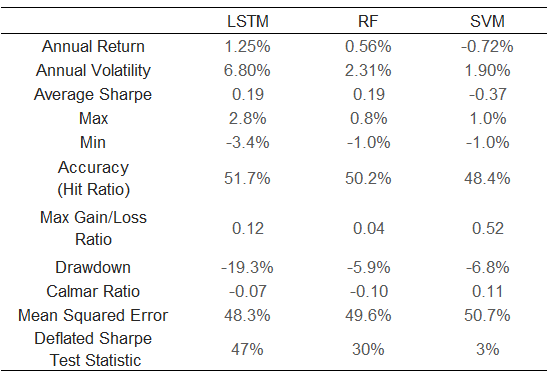
\includegraphics[width=0.6\textwidth]{TrendEstimationSTATSv3}
  %  below is only a naming convention, above is the real deal
    \label{fig:TrendEstimationSTATS}
     \caption*{}
\end{figure}

Figure \ref{fig:TrendFilteredResults}, shows the performance statistics of the models once having been filtered by the trend. The testing period ran from December 2010 until December 2017. The red lines denote the average cumulative performance of all the different trend models created using a particular machine learning model. The blue lines denote the average performance across the models tested of the same strategies when they have been filtered by the trend estimation model. The trend estimation model would reduce the exposure of the trend model to zero if it had predicted a loss in the strategy over the next one month.  

The performance statistics on average across all three models once having been filtered by the trend estimation model are shown in \ref{TrendEstimationSTATS}, on average across all the models, applying trend estimation either increased the average return or reduced a trading strategies' maximum drawdowns (a trading models high to low cumulative losses).

Overall, the two models do tend to work well together and there does seem to be some value in diversifying the decision making process across different models with different specific objectives. Future work in this area could involve a method of transfer learning , where the model trains on the randomly generated data first to recognise the basics of trend, and then train on selected assets which have exhibited trending behaviour so that the model has experienced real world data, finally once these patterns have been learned the trend model could then be tested on the an asset price where the tredn capture model would switch that exposure on and off as the regime changes. 
\clearpage
\subsection{Performance on Blind Test Data}
In this section, we look at the performance of the finalised models and model architectures on a fully unseen set of EURUSD data, this dataset was only used in the last stage of the project to provide an indication of how the model may have performed if it had hypothetically been created at the end of 2017 (when the test data ended). We show the performance of the trend model combined with the trend estimation model. The linear benchmark is shown in red (once again, this is the performance of trading in the direction of the previous 24 hour trend in the currency, \ref{fig:BLINDFULLSYSTEMRES}).
\begin{figure}[h]
    \centering
% below is where you put the acutal image name in the directory
	\caption{Trading System Performance Fully Unseen Live Data}    
	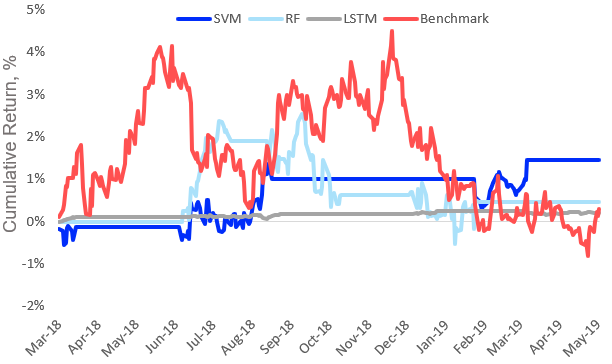
\includegraphics[width=0.6\textwidth]{BLINDFULLSYSTEMRES}
  %  below is only a naming convention, above is the real deal
    \label{fig:BLINDFULLSYSTEMRES}
     \caption*{}
\end{figure}
The model is once again trained on the randomly generated data and then tested on EURUSD price from February 2018 until March 2019 using the same models and specifications as outlined earlier. 
 One clear takeaway is that the machine learning models were much less volatile than the benchmark, and two of the machine learning models outperformed the linear benchmark over the full withheld testing period. While there is not enough data to draw statistical conclusions from the blind test results, there is evidence that the model architecture proposed in this project can indeed be used in the domain of currency trading. The fact that the trend estimation model was able to identity the lack of sustained trend allowed the support vector machine to trade trending price behaviour only when the probability of trend working was high.

The model statistics are shown in \ref{fig:BLINDFULLSYSTEMRES_stats}, the accuracy rates  and mean squared error percentages of the machine learning trend models after applying the model two trend estimation outperforms the linear benchmark for all models. Each machine learning model also outperforms its linear bench mark in terms of the mean annualised returns with lower standard deviation of returns and a vastly reduced drawdown profile.

\begin{figure}[h]
    \centering
% below is where you put the acutal image name in the directory
	\caption{Trading System Performance Fully Unseen Live Data}    
	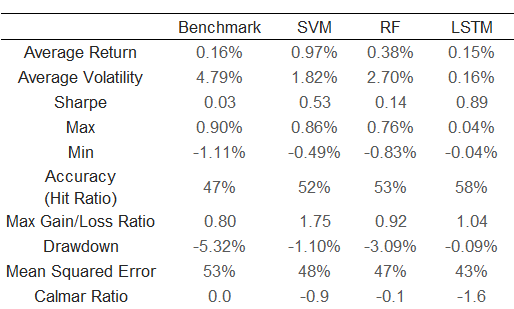
\includegraphics[width=0.6\textwidth]{BLINDFULLSYSTEMRES_statsv2}
  %  below is only a naming convention, above is the real deal
    \label{fig:BLINDFULLSYSTEMRES_stats}
     \caption*{}
\end{figure}


\clearpage


\section{Conclusions} \label{conclusions}

The goal of this project was to assess the applicability of machine learning algorithms in the domain of currency trading. This was done by exploring the most appropriate way in which to use machine learning models to predict currency moves. Initially training the model using historical price data did not perform consistently across different models or features. This is in some way not overly surprising given the inherent heteroskedasticity and efficiency of financial markets. One of the main takeaways of the paper is that we cannot expect machine learning algorithms to perform the heavy lifting of price prediction alone. Financial trading is a multi faceted problem and requires the person developing the trading system to have a deep understanding of the subject domain in order to select and find underlying intuitive reasons to justify the model features or parameter specifications. 
\vspace{4mm}

\par Creating robust models is key to the longevity of a trading model. Overly complicated algorithms will not be able to withstand the test of time in a trading system as they will have over fitted recent history. To try to avoid some of these pitfalls, this paper delegated trading responsibilities to two separate models. Thereby helping to simplify the problem into two distinct problems, one of trend capture and the second of regime identification. Asking the machine learning model to work on one task (identify trend) allows us to simplify the model structure and narrow the number of features used. Predicting trend as opposed to price removes some of the overfitting risk as we are not trying to predict future return based on a host of features, but only find more efficient and accurate ways to capture price momentum. Machine learning models may outperform linear trend models by being able to identify the non-linearities which may help in the early identification of a trend (either beginning or ending). Selecting this trend capture model also allowed us to train the model on randomly generated trending data, which in future could be expanded to allow the model to include transfer learning algorithms which train on both random data and live prices before proceeding to the test stage.
\vspace{4mm}
\par In the second stage of the trading architecture (regime estimation), a random forest model was used to try to understand the complexities between macro-economic data and currency trends. The results presented showcased that the second model was able to identify regimes conducive to the positive performance of trend strategies. Future work in this area could look at adding additional factors such as a mean reversion model to the trend strategy such that the regime estimation model switches between trend and mean reversion based on the probability of a certain regime occurring. Given the simplicity of the model architecture, this type of framework could be scaled up for a multitude of different models which capture various behaviours and various regimes across different asset classes. This project could also be expanded to include new features measuring investor sentiment, positioning, market trading conditions and seasonality. Adding diverse strategies to the model architecture would translate into a higher probability of generalising into the future regardless of the regime.
\vspace{4mm}

\par Overall, the project outlined one way in which machine learning can be used in the domain of financial trading and showcased how separating out duties to two different models can assist in adding robustness to the trading returns.  The results showed promising signs of out of sample success, where the returns were displayed for a host of different strategies and not just the best one.
Machine Learning and artificially intelligent systems will likely see their role in financial markets increase over the course of the next decade as the industry evolves, however in terms of trading algorithms, machine learning methods will remain just one piece of a very large and complex puzzle. There is potential for machine learning methods to outperform standard econometric models however this will still need to be combined with expert domain knowledge, risk management systems, a robust testing framework and data which holds informational value. Above all however, purveyors of the art of financial machine learning will need to remain humble, acknowledge that past performance is rarely an exact guide to the future and that success relies on diversification, hard work and unfortunately...luck.
\clearpage

\bibliography{ref_list}{}
\bibliographystyle{ieeetr} % could also use apalike, ieeetr , abbrv
%\printbibliography
% this moves us to a new page...
\clearpage

\appendix

\section{Appendix}

\subsection{List of Data Files Included in Project}

\begin{table}[h] 
\centering      % used for centering table 
\caption{Data Files Included in Report} % title of Table 
\resizebox{.75\textwidth}{!}{%

\begin{tabular}{l l}  % centered columns (2 columns) 
\hline                     %inserts double horizontal lines 
\hline                     %inserts double horizontal lines 
File Name & Desc. \\ [0.5ex] % inserts table %heading
 \hline                    % inserts single horizontal line 
eurusd\textunderscore hour.csv & EURUSD Hourly Price\\   % inserting body of the table
CurrencyData.csv & G10FX Hourly Price \\ [1ex]
EDI.csv & Econ Data  \\ [1ex]
ESI.csv & Econ Data \\ [1ex]
CcyrandomTrend.csv & Randomly Generated Data \\ [1ex]
CcyrandomTrendLSTM.csv & Randomly Generated Data \\ [1ex]
CcyDataLONGER.csv & Data with Features \\ [1ex]
ccyDataBLIND\textunderscore STFEATURES.csv & Withheld Data Features \\ [1ex]
trendestimation.csv & Data for Trend Estimation \\ [1ex]
trendestimation\textunderscore manual.xlsx & Data for Trend Estimation\\ [1ex]
trendestimation\textunderscore manual\textunderscore BLIND.xlsx & Withheld Data, for Trend Estimation \\ [1ex]
Signals.csv & Raw Signals for Trend Estimation\\[1ex]
Signals\textunderscore blindData.csv & Withheld Data, Raw Signals for Trend Estimation \\[1ex]
Signals\textunderscore FullsamplewBlind.csv & Full Sample Signals For Trend Estimation\\[1ex]
\hline     %inserts single line 
\end{tabular} %
}
\label{table:files} % is used to refer this table in the text 
\end{table} 

\subsection{Code Used in the Project}

\lstinputlisting[language=Python, caption = Code to Generate Random Trending Data]{generate_trend.py}
\lstinputlisting[language=Python, caption = Code to Create Model Features]{create_model_features.py}
\lstinputlisting[language=Python, caption = Code Containing Model Functions]{model_functions.py}
\lstinputlisting[language=Python, caption = Code to Set Parameters of the Models]{run_decision_tree.py}
\lstinputlisting[language=Python, caption = Code to Set Parameters for the Keras \& Tensor flow modules]{ml_trading_module.py}
\end{document}